\documentclass[12pt,a4paper]{extarticle}
\usepackage[a4paper,margin=20mm]{geometry}
\usepackage[french]{babel}
\usepackage[utf8]{inputenc}
\usepackage[T1]{fontenc}
\usepackage{lmodern}
\usepackage{amsmath}
\usepackage{amssymb}
\usepackage{mathrsfs}
\usepackage{fancybox}
\usepackage{graphicx}
\usepackage{wrapfig}
\usepackage{mathabx}
\usepackage{textcomp}
\usepackage{xcolor}
\usepackage{listings}
\newcommand{\ud}{\mathrm{d}}
\newcommand{\hsp}{\hspace{20pt}}
\newcommand{\HRule}{\rule{\linewidth}{0.5mm}}

% Definition de couleur supplementaire
\definecolor{colString}{rgb}{0.6,0.1,0.1}
 
% Definition du langage
\lstdefinelanguage{LangageConsole}{%
    morekeywords={%
        ligne% mot-cl\'{e} ``ligne''
    }
}
 
% Definition du style
\lstdefinestyle{styleLangage}{%
    language        = LangageConsole,%
    basicstyle      = \footnotesize\ttfamily\color{black},% ecriture standard
    identifierstyle = \color{black},%
    commentstyle    = \color{orange},%
    keywordstyle    = \color{blue},%
    stringstyle     = \color{colString},%
    extendedchars   = true,% permet d'avoir des accents dans le code
    tabsize         = 2,%
    showspaces      = false,%
    showstringspaces = false,%
    numbers=left,%
    numberstyle=\tiny\ttfamily\color{black},%
    breaklines=true,%
    breakautoindent=true,%
        backgroundcolor=\color{white},%
}
 
\lstset{%
    style = styleLangage%
}

\begin{document}

%\maketitle
\begin{titlepage}
  \begin{sffamily}
  \begin{center}

    % Upper part of the page. The '~' is needed because \\
    % only works if a paragraph has started.

    \includegraphics[height=4cm]{brain}~\\[1.5cm]

    \textsc{\LARGE Lycée Blaise Pascal Clermont-Ferrand}\\[2cm]
    
    

    \textsc{\Large Dossier TIPE}\\[1.5cm]

    % Title
    \HRule \\[0.4cm]
    { \huge \bfseries Big data, intelligence artificielle et reconnaissance d'espèces marines\\[0.4cm] }

 \HRule \\[2cm]
\begin{minipage}[c]{.46\linewidth}
        \centering
        \includegraphics[height=5cm]{curve}
    \end{minipage}
    \hfill%
    \begin{minipage}[c]{.46\linewidth}
        \centering
        \includegraphics[height=5cm]{CIFAR-10_examples}
    \end{minipage}\\[2cm]
    
    % Author and supervisor
    \begin{minipage}{0.4\textwidth}
      \begin{flushleft} \large
        Maxime \textsc{Cautrès}\\
        Victor \textsc{Bellot}\\
      \end{flushleft}
    \end{minipage}
    \begin{minipage}{0.4\textwidth}
      \begin{flushright} \large
        \emph{Professeurs :} \\
        M. \textsc{Germa}\\
		M. \textsc{Mertens}\\
      \end{flushright}
    \end{minipage}

    \vfill

    % Bottom of the page
    {\large  Octobre 2017 — Juillet 2019}

  \end{center}
  \end{sffamily}
\end{titlepage}


\newpage

\renewcommand{\contentsname}{Sommaire}
\tableofcontents

\newpage

\part*{Abstract}

\textbf{In this document, you will find our temporary solution to the problem of the image recognition, using Deep Neural Networks and a version of the Convolutional Neural Network we developed. We explain both techniques and the back-propagation learning algorithms. We show our way of working, discovering new technologies to improve our results on MNIST and CIFAR datasets. Most of the work was done to make algorithms faster, and to find solutions to the problem of over-fitting which appears with data sets like CIFAR.}


\part*{Introduction }
\bigbreak

\section*{Thème:}

Pour cette première année de classe préparatoire, nous avons eu le plaisir dans le cadre du TIPE de travailler sur un Projet dont le Thème était Océan. C'est un sujet vaste qui ouvrait à de nombreuses problématiques allant des questions environnementales à l'optimisation des routes commerciales, en passant par des problématiques de transports. \'Etant passionnés d'informatique et de mathématiques, nous avons voulu aborder ce sujet à travers la reconnaissance d'images. 

\section*{Problématique:}

Il y a de nos jours de plus en plus d'entreprises telle que Google, Tesla, et bien d'autres qui pratiquent la reconnaissance d'images dans de nombreux domaines,s pour simplifier les recherches sur le net, permettre à des voitures de devenir autonome ou encore faire de la reconnaissance faciale. Lorsque l'on fait des photos sous-marines, il est très difficile pour quelqu'un ne possédant pas de connaissances sur le sujet de savoir ce qu'il photographie; pour répondre à ce problème, nous avons souhaité utiliser la reconnaissance d'images pour permettre l'identification d'une espèce marine seulement grâce à une photographie. Nous allons donc chercher une technologie nous permettant de répondre à la problématique suivante : \textbf{Comment utiliser la grande quantité d'images que l'on peut se procurer aujourd'hui pour permettre l'identification de spécimen marin ?}

\part{Solutions technologiques}

\section{Courte étude de l'existant}

Pour répondre à cette problématique, nous avons regardé les différentes technologies existantes. \textbf{Une première, très naïve, consiste à comparer notre photo à une base de données constituée d'autres photos pour ensuite choisir celle qui ressemble le plus à la notre, et ainsi en déduire l'espèce}. Cette solution possède les désavantages d'\textbf{être extrêmement lente} car pour toute image, elle devra la comparer à une base de données colossale pour que celle-ci soit représentative. De plus, d'autre difficultés liées à la\textbf{ composition de l'image} apparaissent, ce qui limite grandement cette technique au point de la rendre inutilisable. Une autre approche consiste à utiliser \textbf{l'intelligence artificielle}, elle possède de nombreux avantages puisqu'elle \textbf{s'exécute rapidement} une fois entrainée, et n'est pas ou \textbf{peu sensible aux différents problèmes de composition}. Nous avons donc décidé d'utiliser cette technologie. Nous étions déjà en partie familiarisés avec celle-ci à la suite d'un projet déjà en cours. L'intelligence artificielle n'est pas forcement la technologie la plus aisée à mettre en place mais c'est celle qui garantira le meilleur ratio résultat/temps d'exécution une fois celle-ci entrainée. 

\section{Qu'est ce que l'intelligence artificielle ?}

\subsection{Un peu d'histoire}
À la fin du $20^{ème}$ siècle, le créateur de l'ordinateur et le crackeur de la machine de cryptographie \'Enigma,\textbf{ Alan Turing}, pensait déjà qu'un jour les ordinateurs, alors appelés Machine de Turing, arriveraient à battre l'homme dans de nombreux domaines. De son vivant, son génie lui a permis de faire des prévisions sur l'évolution des technologies qui se sont finalement avérées justes. Dans un célèbre article de celui-ci , \textbf{"Computing machinery and intelligence"}, Alan Turing postule qu'un cerveau humain aurait une capacité mémoire d'environ 1 Go, ce qui à l'époque est colossale. Il en conclue qu'il faudrait créer un algorithme d'au minimum 1 Go qui ne se répète pas pour obtenir une complexité équivalente, ce qui serait le résultat de décennies de recherches et encore, sans être certain que la complexité obtenue soit suffisante. \textbf{Il postule qu'il est donc impossible pour l'homme et ses capacités intellectuelles de recréer un cerveau humain adulte. Cependant, il explique qu'il devrait être possible de recréer le cerveau d'un nourrisson, un cerveau "partiellement fini".} Celui-ci est comme vierge, il possède la même structure mais n'a aucune connaissance, aucune logique et donc une complexité bien plus faible car la structure est très simple. L'intelligence artificielle naît de ce postula. Alan Turing n'aura malheureusement pas la chance de voir l'évolution de son travail, puisqu'il meurt prématurément le 7 juin 1954. 
\subsection{Les grandes idées}
Une grande majorité des intelligences artificielles qui ont été créées jusqu'à présent s'inspirent grandement de l'incroyable et perfectionné résultat de l'évolution, notre cerveau. Sa structure est pourtant très simple à comprendre. Le cerveau est un ensemble de neurones plus ou moins connectés entre eux, qui vont modifier un signal électrique porteur d'une l'information. Ce fonctionnement permet de faire émerger des raisonnements extrêmement complexes. \textbf{Cette idée d'émergence est la solution au problème de complexité. }
En mathématiques et informatique, l'émergence qualifie la capacité d'un phénomène très simple à petite échelle à faire apparaitre des comportements extrêmement complexes à grande échelle. On peut par exemple penser au jeu de la vie de Conway qui à partir de lois simples, permet de faire des choses extraordinaire. La complexité qui émerge de ce jeu est telle qu'il a été démontré qu'il est Turing complet, c'est à dire qu'il est possible d'y simuler tout ce qu'on souhaite, même le jeu lui-même. 
\textbf{Pour créer une intelligence artificielle, il faut recréer un cerveau artificiel}; il sera composé de neurones, reliés entre eux par des synapses. Il y aura une entrée d'un côté, et de l'autre une sortie. C'est grâce à cette structure que l'on obtiendra la complexité requise. Mais comment passer de cette structure simple à un algorithme ? Pour cela, il faut s'intéresser aux relations entre les neurones, à l'intérieur de ce réseau. \textbf{Ici, à chaque synapse est associé un nombre, appelé poids. À chaque neurone est associé un nombre, appelé biais. Les poids et les biais du réseau de neurones sont regroupés dans l'ensemble des paramètres du réseau} appelé $\mathcal P$. Maintenant que l'on a exposé ce qu'est un réseau de neurones, nous pouvons nous intéresser à son fonctionnement.

\part{Le Projet}

\section{Les notions:}

\subsection{Les fonctions $F^*$ et $f$}

Maintenant, on sait qu'une intelligence artificielle est un cerveau artificiel, qu'il possède une entrée et on attend de lui qu'il nous ressorte une information, que l'on appellera sortie. De cette description, on peut faire une analogie avec un modèle plutôt familier que l'on retrouve en mathématique, l'application. \textbf{On va donc représenter le cerveau comme une fonction} qui va de l'ensemble des entrées à l'ensemble des sorties \cite{s4a} et \cite{3b1b}. \textbf{L'entrée sera un vecteur (feature) appartenant à l'ensemble des features noté $\mathcal F$, et la sortie (label) sera un vecteur de l'ensemble des labels noté $\mathcal L$}. Pour chaque entrée, on attend une sortie précise qui soit en accord avec l'entrée.\textbf{ On peut donc créer les couples (features, labels) qui sont des points que la fonction doit vérifier}. Ces couples à vérifier peuvent être fournis de différentes manières. Soit avec une \textbf{base de données} qui contient les couples (feature, label), cette option est celle que nous avons choisi pour notre reconnaissance d'images; soit l'algorithme devra de lui même les construire. On ne développera pas les détails de la construction qui ne sont pas utiles dans la réalisation de ce projet, et qui sont très complexes. 
Nous appellerons dès à présent \textbf{$F^*:\mathcal F \mapsto \mathcal L$ la fonction qui vérifie tout les couples (feature, label)} contenus dans la base de données. \textbf{Le but de notre cerveau est d'associer à un feature le bon label}. Ce problème ressemble fortement à celui qu'a résolue Lagrange grâce à ses polynômes interpolateurs. Sauf qu'ici, notre fonction est dans un espaces de bien plus grande dimension et la quantité de points à vérifier est astronomique. C'est pour cela que dans la majorité des cas, \textbf{il n'est pas possible d'avoir une résolution algébrique des inconnues de notre cerveau, qui sont les poids et les biais.} Nous allons donc définir la fonction $f:\mathcal F \mapsto \mathcal L$ qui exécute notre réseau de neurones; elle associe un label à un feature. \textbf{Les images de cette fonction (labels) vont évoluer au cours d'un processus d'apprentissage} qui sera développé plus tard. Il faut cependant savoir qu'\textbf{au début de celui-ci, les poids et biais sont définis aléatoirement}. Le but est, au cours de l'entrainement, d'arriver à \textbf{modifier les paramètres de telle sorte que $f$ approxime au mieux  $F^*$.} \\

Nous pouvons donner ici un exemple de problème où il existe une résolution algébrique: la régression affine. Prenons un neurone; en entrée est présentée l'abscisse d'un point, le poids est un coefficient multiplicatif qui s'appliquera sur l'entrée, le biais est une valeur que l'on ajoute simplement. La fonction $f$ est donc de la forme $f=ax+b=y$. Si l'on veut que notre nuage de point soit le mieux approximé par ce réseau de neurones très simple, il faut calculer $a$ et $b$ grâce à la technique des moindres carrés. L'approximation ne sera pas parfaite car une fonction affine est trop simpliste. Mais on sait trouver les valeurs de $a$ et $b$ qui permettent de minimiser l'approximation.

\subsection{La fonction erreur $E$}

Il nous faut maintenant définir une nouvelle fonction permettant de \textbf{mesurer les performances de $f$}. Comme dit précédemment, les paramètres sont initialement posés aléatoirement. Les images de $f$ seront donc elles aussi aléatoires. Pour mesurer l'erreur entre $f$ et $F^*$ pour un même feature, nous allons nous intéresser à \textbf{la distances $E$ qu'il y a entre le label $Y^*$ qui aurait dû être prédit et le label prédit $y$ par le réseau de neurones}. Pour cela il faut faire un simple calcul de norme avec le produit scalaire canonique de $\mathbb R ^{dimension\ de\ la\ sortie}$:
\begin{equation}
E=(Y^*-y)^2
\label{error}
\end{equation}
Ici, ~\eqref{error} est vectorisée, c'est-à-dire qu'elle calcule la distance entre un certain nombre de $ Y*$ et les $y$ associées. Cela permet de mieux représenter l'erreur du réseau de neurones sans pour autant avoir à recalculer l'erreur sur toutes les données à chaque fois. Cette fonction erreur ne dépend donc pas des features mais seulement des paramètres. Cette fonction aura donc comme ensemble de départ les paramètres de notre réseau de neurones et comme ensemble de sortie une seule valeur, dans $\mathbb R ^+$. D'où $E:\mathcal P \mapsto \mathbb R^+$. \textbf{Pour augmenter les performances de notre cerveau, il nous faudra donc chercher à minimiser l'erreur entre $F^*$ et f, c'est-à-dire, trouver le minimum de $E$}. 

\begin{figure}[h]
        \centering
        \includegraphics[height=6cm]{curve}
        \caption{Représentation d'une fonction erreur quelconque (Surface) avec des chemins la minimisant (Courbes)} \end{figure}

\subsection{L'apprentissage}

Maintenant que nous possédons un moyen de calculer l'erreur de notre réseau de neurones, il faut l'utiliser pour modifier nos paramètres. Ces modifications vont se dérouler durant le processus nommé apprentissage. \textbf{Le réseau de neurones va être testé et ses paramètres seront modifiés plusieurs milliers de fois jusqu'à obtenir une approximation optimale}. Lors de chacun de ces tests, l'erreur sera calculée sur un certain nombre de couples (feature, label), et sera grâce à des formules mathématiques propagée sur les paramètres, ce qui permettra de savoir dans quel sens et avec quelle intensité chaque paramètre devra être modifié. Il sera donc possible de modifier les paramètres et recommencer ce processus autant de fois qu'il sera nécessaire.

\subsection{Les différents types d'algorithmes}

\textbf{Pour la reconnaissance d'images, deux technologies} sont accessibles. \textbf{La première, appelée DNN (pour Deep Neural Network)} sert de base pour \textbf{une seconde appelé CNN (pour Convolutional Neural Network)}. La première utilise un simple \textbf{réseau de neurones profond} pour permettre l'analyse d'une image, alors que la seconde plus complète utilise \textbf{une analyse préliminaire} pour dégager les informations importantes. Nous avons donc décidé de travailler sur ces deux technologies. Ainsi nous pouvons maintenant commencer à aborder notre travail.

\subsection{Les bases de données}
Pour ce projet, nous allons majoritairement utiliser \textbf{deux bases de données}. Une première nommé \textbf{MNIST} \cite{mnist} mise en ligne par Yann LeCun, contenant \textbf{60 000 couples d'images de chiffres écris à la main} (features) avec leur valeur (labels). Cette base de données possède 6000 images pour chaque label ce qui nous donne une belle diversité d'images nécessaire pour l'apprentissage. Cette base de données est\textbf{ un passage incontournable à valider} avant de s'attaquer à d'autres bien plus complexes. La seconde base de données qui sera utilisée est \textbf{extraite CIFAR100 }\cite{cifar}, mise en ligne par l'université de Toronto; elle est composée de 60 000 images classifiées dans 100 catégories. Seule une partie des catégories comporte des images en rapport avec l'océan et les espèces marines. Nous isolerons donc \textbf{une quinzaine de catégories} afin de créer une nouvelle base de données que l'on nommera dès à présent \textbf{CIFAR15}. Il sera bien plus ardu d'avoir une bonne approximation de $F^*$ que pour MNIST car elle possède un nombre plus faible d'images: 600 images par label et un nombre plus important de labels. De plus, les données internes à chaque catégorie sont bien plus variées ce qui complexifie encore la tâche.

\part{Premier algorithme:}


\section{Deep Neural Networks:}
Nous avons donc commencer par utiliser un DNN. Il est la \textbf{clef de voute de l'intelligence artificielle} car il occupe une place majeur dans une grande partie des algorithmes. Généralement il s'occupe de la dernière partie du \textbf{traitement des données} et fournit ainsi les résultats à l'utilisateur. Il est donc incontournable. Cette technologie utilise \textbf{seulement un réseau de neurones}. Il y a plusieurs couches constituées de nombreux neurones. On peut ainsi schématiser un réseau de neurones de la manière suivante: \\


\begin{figure}[h]
        \centering
        \includegraphics[height=6cm]{neural_network}
        \caption{Schéma d'un réseau de neurones}
\end{figure}


Pour simplifier la compréhension, nous allons nous intéresser à ce qu'il se passe pour un neurone isolé. Voici un schéma plus explicite:

\begin{figure}[h]
        \centering
        \includegraphics[height=4cm]{perceptrons}
        \caption{Schéma d'un perceptron (neurone) isolé}
\end{figure}


On y voit ainsi un neurone avec 3 synapses. Cette configuration aura donc 3 poids notés $w_1,w_2,w_3$ respectif à 3 valeurs d'entrées $x_1,x_2,x_3$ et un biais noté $b$. On appelle $a$ la valeur du neurone. La relation mathématique reliant $a$ aux autres variables est la suivante:
\begin{equation}
a = \sigma(x_1\cdot w_1+x_2\cdot w_2+x_3\cdot w_3+b)
\label{compute} \end{equation}
On remarque ici l'apparition d'une fonction $\sigma$ interne à ~\eqref{compute}, il s'agit ici d'une fonction d'activation, elle a pour but d'apporter de la non linéarité au réseau de neurones. Nous détaillerons ceci dans un court instant.  \\
Cette formule permettant de calculer $a$ est unique pour tout le réseau, il faut juste l'adapter en fonction de la taille de chaque couche. Sa variante généralisée est la suivante:
\[a^l_j=\sigma(\sum_k w^l_{jk}\cdot a^{l-1}_k+b^l_j)\]
Ceci étant peut lisible, nous utiliserons une notation:
\begin{equation} a^l=\sigma(w^l\cdot a^{l-1}+b^l) \label{compute_vect} \end{equation}
Voici donc ~\eqref{compute_vect} \textbf{l'unique relation mathématique nécessaire} pour l'exécution d'un réseau de neurones lorsqu'il s'agit d'un DNN.
Il faut maintenant revenir sur \textbf{la fonction d'activation}. Elle peut être de plusieurs types, les plus communes étant les fonctions RELU, tangente hyperbolique, sigmoïde et softmax (détaillée plus tard). Elles ont toutes en commun le fait d'être \textbf{non linéaire}. En effet, le but de notre réseau de neurones est de \textbf{créer de la complexité}, or si on enlève les fonctions d'activations, les relations mathématiques internes au réseau ce \textbf{résumeront en une seule et unique combinaison linéaire} des valeurs d'entrées, ce qui n'est clairement pas souhaitable car cela réduirait toute la complexité de notre algorithme. Ainsi ces fonctions d'activations sont des éléments clefs du bon fonctionnement du DNN. Il nous faut donc maintenant définir les relations mathématiques utiles à l'algorithme d'apprentissage. 


\section{Evolution de l'algorithme}

\subsection{Découverte de la technologie}

Maintenant que nous possédons le cerveau artificiel, il faut l'entrainer. Nous avons souhaité commencer avec un \textbf{algorithme de descente de gradient}. La technologie est accessible et sa mise en place aisée. Pour savoir comment il faut modifier chaque paramètre, on va chercher leur \textbf{influence individuelle sur l'erreur}. Pour cela, on calcule l'erreur avec une première version de nos paramètres, et on va ensuite modifier un poids en lui ajoutant une petite valeur $\epsilon$. Puis on calcule à nouveau l'erreur et on la compare à l'ancienne, si celle-ci est supérieure, c'est que la modification est néfaste, et donc qu'il faut effectuer la modification inverse. Au contraire si cette modification diminue l'erreur, on peut la considérer comme bénéfique, et donc la conserver. Lorsque l'on effectue ce processus sur tout les paramètres du réseau, poids et biais, on réduit de manière importante l'erreur de notre notre réseau de neurones.\textbf{ Au fur et à mesure des itérations, les poids et les biais définis initialement de manière aléatoire vont évoluer jusqu'à tendre vers des valeurs minimisant l'erreur}. Dans cet algorithme, il faut donc choisir la valeur de $\epsilon$. Nous avons choisi $\epsilon = 10^{-5}$, une valeur assez importante pour pouvoir rapidement converger vers une solution, mais pas trop élevée, ce qui aurait pu empêcher l'algorithme de converger. On aperçoit déjà ici \textbf{de nombreuses limites} à notre algorithme. Le fait que nous ayons à choisir un pas fixe ralentit l'entrainement au début et l'empêche d'obtenir des résultats très précis sur la fin. De plus, le pas de modification $\epsilon$ est le même pour tout les paramètres, donc l'entrainement n'est pas forcement optimal. L'algorithme met aussi \textbf{un temps très important} pour atteindre des résultats cohérents car il doit faire un nombre très important de modifications sur chaque paramètre avant de converger. Or chaque modification de paramètre implique deux calculs d'erreur qui nécessitent d'exécuter l'entièreté du réseau. \textbf{Sur la base de donnée MNIST, nos résultats était 60\% de réussite, ce qui est faible pour cette base de données}. Nous sommes donc partis en quête d'un nouvel outil, plus efficace, pour nous permettre d'obtenir de meilleures performances.

\subsection{Familiarisation avec la rétro-propagation}

\subsubsection{Les notations}

Cette solution, nous l'avons trouvée après de nombreuses recherches sur le Net: il s'agit de l'\textbf{algorithme de rétro-propagation} \cite{steve}. Il va limiter un maximum les calculs en cherchant à minimiser le nombre de fois où l'on ré-exécute le réseau de neurones. Ici, on va utiliser les mathématiques, et grâce à des relations \textbf{on va propager l'erreur sur tous les neurones, les poids et les biais}. Cela nous permettra d'avoir à calculer une seule fois l'erreur pour ensuite modifier les paramètres. 

\begin{figure}[h]
        \centering
        \includegraphics[height=6cm]{curve2}
        \caption{\textbf{En rouge:} Descente de gradients conventionnelle très directe mais lente. \textbf{En noir:} Exemple de rétro-propagation, moins directe mais bien plus rapide.}
\end{figure}

Pour arriver à cela, il faut faire des mathématiques. Le but de cette partie est de \textbf{trouver des relations permettant de faire reculer l'erreur dans les neurones} et ainsi obtenir pour chacun des paramètres leur influence sur l'erreur.
Il va donc falloir définir plusieurs relations. Commençons par introduire les notations de nos neurones, poids ,biais et autres paramètres:
\begin{itemize}
\item La valeur d'un neurone est notée $a^l_n$ pour le $n$-ième neurone de la $l$-ième couche.
\item Un poids est notée $w^l_{n,m}$ pour le poids du $n$-ième neurone de la $l$-ième couche qui s'applique sur le neurone $m$ de la $(l-1)$-ième couche.
\item Un biais est notée $b^l_n$ pour le biais du $n$-ième neurone de la $l$-ième couche.
\item On défini $z$ de la manière suivante : 
\begin{equation} z^l_n=\sum_k a^{l-1}_k\cdot  w^l_{n,k}+b^l_n \label{z} \end{equation} 
\item On a donc $a^l_n=\sigma(z^l_n)$ où $\sigma$ est une fonction d'activation.
\end{itemize} 

\subsubsection{Les équations mathématiques}
Maintenant que nous avons présenté les notations, il est possible de travailler sur les équations. Il faut d'abord obtenir \textbf{l'influence de la sortie sur l'erreur:} \\
Pour cela rappelons notre fonction $E$:
\[E=(Y^*-y)^2\Leftrightarrow E = <(Y^*-y)|(Y^*-y)> \Leftrightarrow E = \sum_k(Y^*_k-a^L_k)^2 \]

Grâce à cette écriture on peut, en utilisant les \textbf{dérivées partielles}, calculer l'\textbf{influence de chaque paramètre} et valeur de notre réseau sur l'erreur. Cela permet donc d'en déduire les formules suivantes (les preuves sont détaillées dans l'annexe):

\begin{align}
\ud a^L_k&=a^L_k-2Y^*_k\\
\ud z^l&= \sigma'(z^l) \circ \ud a^l \\
\ud a^{l-1}&=T_{w^l}\cdot \ud z^l\\
\ud w^l&=\ud z^l\cdot T_{a^{l-1}}\\
\ud b^l&=\ud z
\end{align}

Maintenant que nous possédons l'influence des poids et des biais sur l'erreur, il est possible de les modifier pour ainsi réduire l'erreur. Tout \textbf{les paramètres seront donc redéfinis de la façon suivante}:
\[w^l_{n,m} - \alpha\cdot \ud w^l_{m,n}\mapsto w^l_{n,m}\]
\[b^l_n - \alpha \cdot \ud b^l_n \mapsto b^l_n\]
Ici, $\alpha$ est le learning rate, valeur arbitraire que nous définissons nous même au début de l'entrainement. Elle est de l'ordre de $10^{-3}$. Grâce à ces relations, \textbf{on possède le strict  minimum pour procéder à un entrainement.} \\

\subsubsection{Les mini-batchs}
Il y a cependant \textbf{quelques modifications à apporter} au fonctionnement de notre algorithme; pour accélérer son exécution, on peut introduire le concept de mini-batchs. \textbf{Un mini-batch est un groupement de features} traités en parallèle grâce à la vectorisation. Cela va nous permettre de faire tout les calculs en une seule fois en considérant le vecteur de features du mini-batch.  Cela va ajouter une dimension à toutes nos données, et par des choix astucieux dans les arguments des fonctions numpy (librairie python de calculs matriciels), nous allons pouvoir conserver les mêmes expressions mathématiques pour l'exécution et la rétro-propagation avec ou sans mini-batchs. Il nous faut préalablement définir de nouvelles notations prenant compte des mini-batchs:
\[a^{l,i}_{n},z^{l,i}_{n},b^{l,i}_{n},w^{l,i}_{n,m},\ud a^{l,i}_{n},\ud z^{l,i}_{n},\ud b^{l,i}_{n},\ud w^{l,i}_{n,m}\]
Nous pouvons donc maintenant définir deux nouvelles notations:
\begin{itemize}
\item Les gradients pour les poids:
\[gw^l_{n,m}=<\ud w^{l,i}_{n,m}>_i\]
\item Les gradients pour les biais:
\[gb^l_{n}= <\ud b^{l,i}_n>_i\]
\end{itemize}

Les paramètres seront donc redéfinis de la manière suivante:
\begin{equation} w^l_{n,m} - \alpha \cdot gw^l_{m,n}\mapsto w^l_{n,m} \label{up_w} \end{equation}
\begin{equation} b^l_n - \alpha \cdot gb^l_n \mapsto b^l_n \label{up_b} \end{equation}

\subsubsection{L'algorithme d'apprentissage:}

Maintenant que nous possédons les équations, il ne nous reste plus qu'à créer un protocole d'apprentissage.
\begin{itemize}
\item Il faut \textbf{créer les mini-batchs}: pour cela il reste une dernière étape de manipulation des données. Nous avons notre base de données sous formes d'une très grande liste de couple (feature, label). Il nous faut la séparer en \textbf{deux listes que l'on nommera Train et Test}, puisqu'il nous faut des données pour permettre au réseau de neurones d'apprendre puis des données pour tester celui-ci. Ces tests doivent s'effectuer sur \textbf{des données qui lui sont inconnues} pour pouvoir mesurer ses performances dans une utilisation réelle: les images de chiffres ou de poissons que l'on voudra reconnaître ne peuvent pas être dans la base de données lors de l'entrainement. Nous séparons donc en mettant $85\%$ des données dans la liste Train et les $15\%$ restant dans la liste Test.
\item Maintenant que l'on possède une liste de données pour l'entrainement, il faut la séparer en mini-batchs de taille n. Pour cela, on \textbf{mélange notre liste Train puis l'on sépare la liste en plusieurs mini-batchs.} La taille des mini-batchs ne divisant pas forcément celle de la base de données, il y aura dans la majorité des cas un mini-batch avec moins de données que les autres. Nous décidons de ne pas le considérer pour l'entrainement.

\item Nous pouvons donc commencer un entrainement. Pour chaque mini-batch, \textbf{l'algorithme va exécuter le réseau de neurones et sauvegarder les matrices de valeurs $a$ et $z$}. 
\item Il va ensuite \textbf{calculer $E$}.
\item Il va \textbf{rétro-propager l'erreur} à travers l'entièreté du réseau de neurones grâce aux 4 équations pour \textbf{obtenir $\ud a,\ud z,\ud w$ et $\ud b$}.
\item Il va \textbf{calculer les gradients $gw$ et $gb$}.
\item Et il finira par \textbf{mettre à jour $w$ et $b$}
\end{itemize}

Ce processus est répété autant de fois qu'il y a de mini-batchs. Une fois tout les mini-batchs utilisés, il reste à regarder les \textbf{performances de l'algorithme sur la liste Test}. On calcule donc son pourcentage de succès, c'est-à-dire le nombre de bonnes prédictions sur le nombre d'éléments de Test. \textbf{On appelle époque l'ensemble de ce processus d'apprentissage sur un unique set de mini-batchs}. Pour améliorer les performances, il faut faire plusieurs époques. Un entrainement complet est donc l'exécution de plusieurs époques (avec à chaque itération des mini-batchs différents grâce au mélange au début de l'époque) sur un même cerveau. Ceci est donc la base de la rétro-propagation. Il existe encore cependant des façons d'améliorer cette technologie. 

\subsection{Algorithme final} 

\subsubsection{Fonctions d'activations}
Maintenant que nous savons précisément ce qu'est une rétro-propagation et comment l'intégrer à notre réseau de neurones, nous pouvons nous intéresser à d'autre \textbf{outils qui permettent d'accélérer la convergence} lors de l'entrainement.
Nous allons tout d'abord présenter les différentes fonctions d'activation que nous avons souhaitées utiliser et les petites modifications que celles-ci peuvent engendrer.
\begin{itemize}
\item \underline{La Sigmoïde}. Il s'agit de la fonction d'activation \textbf{la plus connue}, elle est de la forme $\sigma(z)=\frac{1}{1+e^{-z}}$ de dérivée $\sigma'(z)=\sigma(z)\cdot (1-\sigma(z))$. Elle fournie des valeurs entre 0 et 1 et est non linéaire. Elle possède donc les caractéristiques d'une fonction d'activation mais elle possède \textbf{un principal défaut, l'utilisation d'une exponentielle}. En informatique, l'opérateur exponentiel est très lent, donc l'utiliser des millions de fois lors de chaque entrainement va engendrer \textbf{une perte de temps conséquente}, c'est pour cette raison que nous avons rapidement \textbf{décidé de ne plus l'utiliser}.
\item \underline{La tangente hyperbolique} de dérivée $\tanh'(z) = 1 - \tanh^2(z)$. Cette fonction possède des \textbf{caractéristiques similaires à la sigmoïde}, elle est croissante, avec son image comprise entre $-1$ et $1$. Elle est aussi une bonne fonction d'activation, mais elle possède les \textbf{mêmes défauts temporels que la sigmoïde}, donc nous avons décidé de ne pas l'utiliser.
\item \underline{La fonction RELU} de la forme $\sigma(z)=z^+=max(z,0)$. Sa dérivée est de la forme $\sigma'(z)=\frac{max(0,z)}{|z|}=\frac{RELU(z)}{|z|}$. Cette fonction va dans $\mathbb R^+$ et est non linéaire. Elle possède \textbf{l'avantage d'être très légère à calculer}, et ce même pour sa dérivée. Elle est donc \textbf{idéale} pour la grande quantité de calculs où celle-ci va être utilisée. Par conséquent \textbf{elle sera utilisée dans la grande majorité des cas}.
\item \underline{La fonction Softmax}. Celle-ci est \textbf{très spécialisée}, elle s'utilise seulement sur la \textbf{dernière couche}. Elle est particulière dans le fait qu'elle nécessite de connaître toutes les valeurs de la dernière couche. Elle s'exprime ainsi :
\[\sigma(z^L_n)=\frac{e^{z^L_n}}{\sum_k e^{z^L_k}}\] 
Cette fonction d'activation map les valeurs de sortie entre 0 et 1 \textbf{de manière exponentielle}. Cela nous permet de pouvoir plus facilement comparer nos résultats avec les labels car cette fonction \textbf{dilate les écarts} entre les valeurs basses et élevées du vecteur de sortie (aspect exponentiel). De plus \textbf{la somme des composantes du vecteur sortie sera 1, cela pourra nous permettre d'approximer la sortie à un vecteur de probabilité.} Cette fonction d'activation nous oblige ainsi à modifier notre définition de $\ud a^L$ et de $dz^L$. La définition de $ \ud a^L$ n'est plus nécessaire et l'on trouve directement $\ud z^L$ grâce à la relation suivante: 
\[\ud z^L_k=\frac{1-Y^*_k}{1-a^L_k}-\frac{Y^*_k}{a^L_k}\]
Ici la division et l'addition sont des opérateurs termes à termes.
\end{itemize}



\subsubsection{Les optimiseurs}

Il faut maintenant introduire les optimiseurs \cite{optimiseur1}. Dans notre algorithme précédemment présenté, \textbf{seuls les gradients calculés lors d'un seul mini-batch sont utilisés pour modifier les paramètres}. Cependant, il existe des \textbf{manières plus optimales de procéder} pour modifier les paramètres. Le principales sont les suivantes:\textbf{ RMSprop, Momentum et Adadelta}. Nous allons expliquer en détail ces 3 optimiseurs:
\begin{itemize}
\item \underline{RMSprop} pour Root Mean Squared  prop. Cet optimiseur utilise de nouvelles variables supplémentaires que l'on nomme $p$, $q$, $gp$ et $qgp$ avec $p$ notre matrice des paramètre, $qg$ la matrice des gradients des paramètres, et $qgp$ une sauvegarde de la dernière matrice de gradients calculée, et l'on à les relations mathématiques suivantes:
\[q^l=\gamma \cdot qgp^l+(1-\gamma)(gp^{l})^2\]
\[p^l - \alpha \frac{gp^l}{\sqrt{q^l+\epsilon}}\mapsto p^l \]
\[qgp^l = q^l \]
RMSprop va influer les gradients calculés en fonction de ceux précédemment calculés, cela va apporter un \textbf{petite inertie }grâce au paramètre $\gamma$. ici $\epsilon = 10^{-6}$
Après de nombreux tests, nous nous sommes rendu compte que cet optimiseur est bien moins efficaces que les deux suivants. 

\item\underline{Le Momentum} est un optimiseur qui va apporter \textbf{beaucoup d'importance aux modifications passées}. Il va utiliser, comme le RMSprop, une sauvegarde, mais celle-ci ne permettra pas seulement d'augmenter plus ou moins la norme de $gp$, elle \textbf{influera même sur direction} de $gp$ en mettant une certaine inertie dans la direction des modifications. Donc si les paramètres sont modifiés dans la bonne direction, cela va confirmer la direction. Il est possible qu'un petit nombre de gradients demandent des modifications inverses, or grâce à cet optimiseur, ils seront négligés grâce à l'inertie s'il s'avère que cette modification de direction était seulement passagère, mais elle seront prises en compte si la modification de trajectoire devient plus importante. Le paramètre nous permettant de gérer l'inertie est $\beta$. Intéressons-nous maintenant aux équations:
\[q^l=\gamma\cdot qgp^l+(1-\gamma)gp^l\]
\[p^l - \alpha \cdot q^l \mapsto p^l \]
\[qgp^l = q^l \]

\item \underline{L'Adadelta}, il possède les avantages du momentum et la caractéristique d'augmenter grandement la norme du vecteur gradient quand celui-ci confirme la direction des gradients des mini-batchs précédents. Cela permet \textbf{encore d'accélérer l'apprentissage} car il se déplacera plus vite. Son expression mathématique est complexe, elle ne sera donc pas évoquée ici. 

\end{itemize} 

\textbf{Nous allons utiliser alternativement les deux derniers optimiseurs} au cours du projet, voici des liens \cite{optimiseur2} et \cite{optimiseur3} pour des animations illustrant visuellement les différences de performances.

\subsubsection{Le Drop out et principe de sur-apprentissage}

Une dernière amélioration que l'on peut intégrer est appelée \textbf{Drop Out}. Cela va permettre de \textbf{réduire la différence entre l'erreur obtenue sur les Tests et la seconde sur les Trains}. Effectivement, notre réseau de neurones a été entrainé sur un certain nombre de données dont il a connaissance, mais nous souhaitons savoir ses performances sur des données qui lui sont inconnues. On juge la capacité d'un réseau de neurones à extraire la sémantique des images qu'il a analysées. \textbf{S'il possède un pourcentage de réussite très important sur les Train mais bien plus faible sur les Test}, nous pouvons conclure qu'il a \textbf{appris par cœur les données} d'entrainement. Il ne sait donc pas extraire la sémantique des images et sera donc \textbf{moins performant quand il ne connaîtra pas les images} sur lesquels il sera testé. \textbf{Ce phénomène nommé sur-apprentissage} est très présent pour les bases de données avec \textbf{peu d'images pour chaque label} et plus généralement peu d'images tout labels confondus. Pour limiter le sur-apprentissage, on peut utiliser le \textbf{drop out}: cela consiste à \textbf{handicaper l'algorithme en le privant de certain de ses neurones durant l'entrainement}, ce qui a pour conséquences de l'obliger à s'adapter à des situations jusqu'alors inconnues. Plus précisément, le drop out va permettre de \textbf{dédoubler un certain nombre de calculs internes} au cerveau. Par exemple, si un seul neurone fait tout le travail et qu'il se retrouve éteint, l'algorithme va en adapter d'autres pour le remplacer, cela permet ainsi quand on le rallumera d'avoir \textbf{multiplié le nombre de neurones permettant d'obtenir le résultat}. Or, ce sont les probabilités qui nous le disent, dédoubler les tests permet grandement de limiter les erreurs. À la fin de l'entrainement, \textbf{on lui redonne pleine capacité sur des images inconnues et on voit une diminution de l'écart de performance entre Tests et Trains}. Cette diminution confirme l'importance d'effectuer plusieurs fois le même test. Pour désactiver un certain nombre de neurones, on va générer une matrice de même format que $a^{:L}$ contenant des $1$ et l'on va mettre dans chaque layer l des valeurs à $0$ avec une probabilité de $Dor^l$ (Drop out rate). Ensuite nous multiplierons à un moment précis chaque valeurs par son coefficient associé dans cette matrice, ce qui aura comme conséquence de désactiver le neurone si la valeur est 0 ou l'activer si la valeur vaut 1. Cependant, cette technologie possède le désavantage de beaucoup \textbf{réduire les performances du réseau sur les trains}, l'apprentissage étant plus long et les résultats moins bons. Cette technologie est aussi \textbf{délicate à mettre en place} car mal intégrée à l'apprentissage, elle peut le rendre impossible. Il nous faudra donc trouver une nouvelle optimisation pour rehausser les performances. Pour exemple, les \bsc{Figure 5 et 6} montrent des courbes d'évolutions de l'erreur sans drop out et avec un drop out mal placé. \\

\begin{figure}[h]
    \begin{minipage}[c]{.46\linewidth}
        \centering
        \includegraphics[height=4.5cm]{Perfect}
        \caption{Évolution de l'erreur durant l'apprentissage sans Drop Out}
    \end{minipage}
    \hfill%
    \begin{minipage}[c]{.46\linewidth}
        \centering
        \includegraphics[height=4.5cm]{drop_out_de_merde}
        \caption{Évolution de l'erreur durant l'apprentissage avec Drop Out mal implémenté }
    \end{minipage}
\end{figure}

 
\section{Résultat}

Maintenant que nous avons un algorithme, nous pouvons parler de \textbf{ses performances}. Tout d’abord la base de données \textbf{MNIST}, composée de $60 000$ couples, a été séparée en deux: $50 000$ pour l’apprentissage et $10 000$ pour les tests. Ici, les images sont au format $28\times 28$ en nuances de gris. Cela donne $784$ neurones sur la couche d'entrée, un par pixel. Puisqu'il y a $10$ labels différents, le réseau aura besoin de $10$ neurones sur la couche de sortie. Pour augmenter la complexité, nous avons choisi, après de nombreux tests, une couche intermédiaire entre la couche d'entrée et de sortie de $64$ neurones, ce qui optimisait les performances par rapport au temps. Cela amène à une \textbf{configuration avec $50 816$ poids et $74$ biais} pour un nombre total de $50 890$ paramètres à entrainer. \textbf{Sans optimiseurs, sans drop out} et avec les fonctions d'activations, nous avons atteint les \textbf{$94\%$ de réussite sur les Trains et $89\%$ sur les Tests}. Lorsque l'on rajoute les \textbf{optimiseurs, on peut atteindre les $100\%$ de réussite sur les Trains et $94.5\%$ sur les Test}. En utilisant le \textbf{drop out}, nos performances sur les \textbf{Trains ont réduit à $99.1\%$ mais celle sur les Tests on augmenter avec $96.1\%$}. 

\begin{figure}[h]
    \begin{minipage}[c]{.46\linewidth}
        \centering
        \includegraphics[height=5cm]{fin_du_game}
        \caption{Résultat du meilleur entrainement sans drop out sur MNIST (100\% et 94.5\%)}
    \end{minipage}
    \hfill%
    \begin{minipage}[c]{.46\linewidth}
        \centering
        \includegraphics[height=5cm]{retour_aux_sources}
        \caption{Résultat du meilleur entrainement avec drop out sur MNIST (99.1\% et 96.1\%)}
    \end{minipage}
\end{figure}

Nous nous sommes intéressés à \textbf{l'influence du drop out sur l'entrainement}, les courbes obtenues ci-dessous représentent l'évolution des performances avec différents taux de drop out à plusieurs endroits du réseau.

\begin{figure}[h]
        \centering
        \includegraphics[height=8cm]{dor_compare}
        \caption{Courbes de performance en fonction des taux de drop out}
\end{figure}


Les courbes présentées sur les images sont les \textbf{courbes d'évolution de l'erreur sur les Trains (bleue) et les Tests (rouge)} au cours des époques d'entrainements. On voit clairement, grâce aux courbes qui se séparent de plus en plus au fils des itérations, que notre algorithme a \textbf{un sur-apprentissage important}. On voit aussi \textbf{des différences au niveau du lissage de la courbe} en fonction du \textbf{taux de drop out. Plus celui-ci est important, plus les courbes sont chaotiques}, cela est dû au fait que le drop out déstabilise l'algorithme en désactivant de façon aléatoire un certain nombre de neurones. On voit aussi qu'il y a \textbf{peu ou pas de variation des taux de sur-apprentissage} en fonction du drop out, cela montre donc la faible influence du drop out sur l'écart. Une technologie permet de rendre le drop out bien plus efficace, elle sera intégrée plus tard. Mais une \textbf{très faible variation au niveau de l'erreur va se ressentir grandement au niveau des pourcentages de réussites}. C'est pour cela que nous avons tout de même pu avoir une amélioration de $2\%$ sur les Tests.  \\

Nous souhaitons maintenant utiliser \textbf{CIFAR15} comme base de données pour notre réseau de neurones. Celle-ci comporte des \textbf{images bien plus lourdes en $32\times32\times 3$ RGB}. Si l'on veut conserver une configuration similaire à une couche intermédiaire, cela nous porte à $3072$ neurones pour l'entrée, $64$ pour la couche intermédiaire et $15$ pour la finale. Cependant, d'après nos tests, la complexité permise par cette configuration n'est pas assez importante pour cette base de données , nous avons donc décidé après d'autres tests de rajouter une seconde couche intermédiaire située directement après l'entrée avec $784$ neurones. Cela nous fait \textbf{$2 459 584$ poids et $863$ biais}, ce qui porte à $2 460 447$ le nombre de paramètres \textbf{à entrainer}. Cette énorme quantité de paramètres à entrainer rend notre \textbf{algorithme} presque \textbf{inutile} puisqu'il lui faut u\textbf{n temps très important pour commencer à converger et ensuite tendre vers des résultats acceptables}. Nous avons donc rapidement \textbf{oublié cet algorithme pour répondre à nos besoins }et avons cherché \textbf{une nouvelle technologie plus appropriée à la reconnaissance d'images: les réseaux de neurones de convolution.} 



\part{Second algorithme}
\section{Convolutional Neural Networks:}
Les \textbf{réseaux de neurones de convolution} \cite{cnn} sont l'évolution logique des réseaux de neurones profonds que l'on utilisait jusqu'alors. Cette technologie, que l'on nommera \textbf{CNN}, utilise un \textbf{DNN classique}, mais ce, \textbf{parée d'une première étape de modifications des images}, qui sera elle aussi entrainable. Elle aura pour but de condenser les informations contenues dans l'image initiale dans une image de bien plus petite dimension. Pour cela il nous faut introduire le \textbf{principe de filtrage par convolution}. Le filtrage par convolution est une technologie utilisée pour faire \textbf{ressortir certaines caractéristiques d'une image}. Elle s'appuie sur le principe de \textbf{produit de convolution entre une image et un masque}, l'image et le masque étant sous forme matricielle. Le fonctionnement est le suivant: on prend une matrice $k$ de taille $n \times m$. On fait le produit membre à membre des éléments de $k$ avec un bloc de format $n\times m$ extrait de l'image et de coordonnées de l'angle supérieur gauche $(x,y)$. Une fois le produit d'Hadamard effectué, il faut sommer toutes les valeurs de la matrice obtenue. Cette somme sera assignée à la coordonnée $(x,y)$ de la nouvelle image. Cette opération va ensuite être effectuée sur l'ensemble des pixels de coordonnées $(x,y)$ de l'image d'entrée, ce qui donne une nouvelle image correspondant à l'image initiale passée par le filtre. Il existe des \textbf{matrices précises qui ont des rôles déterminés}. Par exemple :
\begin{itemize}
\item La matrice 
$\begin{bmatrix} 
-1 & -1 & -1 \\
-1 & 8 & -1 \\
-1 & -1 & -1  
\end{bmatrix}$ permet par un produit de convolution de \textbf{faire ressortir les contours des objets} d'une image.
\item La matrice
$\frac{1}{16}\cdot \begin{bmatrix}
1 & 2 & 1 \\
2 & 4 & 2 \\
1 & 2 & 1 
\end{bmatrix}$ \textbf{applique un flou} sur l'image d'entrée.
\end{itemize}
Ces deux matrices sont deux exemples issus de la diversité des filtres existant. \textbf{On peut cependant se demander comment intégrer ces filtres à un réseau de neurones en sachant qu'il est impossible de savoir quels filtres seront utiles à notre algorithme}. Il faudra donc trouver une manière de les déterminer.
Un CNN, pour Convolutional Neural Network, va être en deux parties. Une première qui utilisera les convolutions et une seconde qui utilisera un réseau de neurones. \textbf{La seconde partie est similaire en tout point à notre premier algorithme.} Il faut donc s'intéresser à la partie \textbf{convolutions}:
Elle est composée de \textbf{plusieurs couches de filtres}; nous allons considérer une de ces couches pour introduire les notations, le fonctionnement, et les formules.
\begin{figure}[h]
\centering
\includegraphics[width=16cm]{CNNlayer}
\caption{Lien entre deux couches du réseau de convolution.}
\end{figure}
On voit qu'il y a \textbf{deux étapes} pour chaque couche de convolution. Une première consiste en l'\textbf{application du produit de convolution}, et une seconde appelée pooling sert à \textbf{réduire la dimension de l'image}.
\begin{itemize}
\item Commençons par la convolution. Il faut déjà comprendre \textbf{comment appliquer un filtre appelé kernal sur une image}. Utilisons un schéma pour appuyer l'explication:
\begin{figure}[h]
\centering
\includegraphics[height=3cm]{CONVO}
\caption{Exemple de calcul d'un produit de convolution.}
\end{figure}\\
\begin{align}
0&=-16-3-2-10-11-9-6-7+8\times 8 \\
0&=-1-6-7-8-10-11-14-15+9\times 8 \\
30&=-2-3-5-6-8-9-12-13+8\times 11 \\
-30&=-4-5-8-9-11-12-14-15+8\times 6 
\end{align}
Dans la grande majorité des cas, les images sont sur 3 dimensions en non deux, les filtres auront donc 3 dimensions. Il faut donc trouver une écriture mathématique du produit de convolution en 3 dimensions, mais il nous faut avant définir les notations. Soit $A^l_{w,h,d}$ le pixel de coordonnées $(w,h,d)$ de l'image d'entrée $A^l$ de format $(W^l,H^l,D^l)$, soit $K^l_{w,h,d}$ la valeur de coordonnées $(w,h,d)$ du filtre $K^l$ de format $(kw^l,kh^l, kd^l=D^l)$. Soit $Z^l_{w,h,d}$ le pixel de coordonnées $(w,h,d)$ de l'image de sortie $Z^l$ de format $(W^l-kw^l+1, H^l-kh^l+1, 1)$. On a donc l'égalité suivante:
 

\[ \forall (w,h,d)\in \ldbrack 0,W^l-kw^l\rdbrack \times \ldbrack 0, H^l-kh^l\rdbrack \times \{0\},\]
\[ Z^l_{w,h,0}= \sum_{\begin{array}{c} aw\in \ldbrack 0, kw^l-1\rdbrack \\ ah\in \ldbrack 0, kh^l-1\rdbrack \\ ad\in \ldbrack0,kd^l-1\rdbrack \end{array}}K^l_{aw,ah,ad}\cdot A^l_{w+aw,h+ah,ad} \]

Or pour \textbf{augmenter le pouvoir d'analyse des filtres}, on va appliquer un nombre $kc^l$ de filtres qui dépend de la couche. Il faut donc rajouter un indice à certaines nos notations :
\[K^{l,n}_{w,h,d}, Z^{l}_{w,h,d}\]
On a donc le format de $Z^{l}$ qui vaut $(W^l-kw^l+1, H^l-kh^l+1, kc^l)$, d'où la nouvelle équation:

\[ \forall (w,h,d)\in \ldbrack 0,W^l-kw^l\rdbrack \times \ldbrack 0, H^l-kh^l\rdbrack \times \ldbrack 0,kc^l-1 \rdbrack,\]
\begin{equation}
 Z^{l}_{w,h,d}= \sum_{\begin{array}{c} aw\in \ldbrack 0, kw^l-1\rdbrack \\ ah\in \ldbrack 0, kh^l-1\rdbrack \\ ad\in \ldbrack 0,kd^l-1 \rdbrack  \end{array}}K^{l,d}_{aw,ah,ad}\cdot A^l_{w+aw,h+ah,ad}
\label{CNN} 
\end{equation}
\item Il faut donc maintenant \textbf{justifier de la nécessité de la seconde partie d'une couche de convolution}. Elle est composée d'une \textbf{fonction d'activation et d'un pooling}. La \textbf{fonction d'activation} s'occupe toujours d'apporter de \textbf{la non linéarité} pour rendre les calculs finaux irréductibles, ce qui permet de conserver une complexité élevée. Il reste donc à détailler le fonctionnement du pooling. Il faut rappeler que \textbf{l'intérêt d'un réseau de convolution est d'avoir des images plus légères à l'entrée du DNN pour limiter le nombre de poids et de biais}, \textbf{il faut donc réduire le nombre de pixels de notre image à chaque étape.} C'est ici qu'intervient le pooling: il va s'appliquer de \textbf{différentes manières}, comme le montre l'image qui suit:  
\begin{figure}[h]
\centering
\includegraphics[width=16cm]{Pooling}
\caption{Illustrations selon 3 fonctions de pooling}
\end{figure}
On voit ici une logique apparaître: premièrement, après avoir fait passer notre image $Z^l$ dans une fonction d'activation, on obtient une nouvelle image $Z'^l$ de même format $(W'^l,H'^l,D'^l)$. Il va falloir \textbf{quadriller l'image en rectangle }de format $(pw^l,ph^l)$ pour leur \textbf{associer leur moyenne, leur maximum ou leur minimum} que l'on notera $\Phi$. L'ensemble des valeurs associées à l'image $Z'^l$ est $A^{l+1}$
Établissons les relations mathématiques:

\[ \forall (w,h,d)\in \ldbrack 0,\left\lfloor \frac{W'^l}{pw^l} \right\rfloor -1 \rdbrack 
\times \ldbrack 0, \left\lfloor \frac{H'^l}{ph^l} \right\rfloor -1\rdbrack \times \ldbrack 0,D'^l-1 \rdbrack,\]
\begin{equation}
A^{l+1}_{w,h,d}=\Phi\left( ( Z'^l_{x,y,d})_{
\left\{\begin{array}{l}
x \in \ldbrack w\cdot pw^l, (w+1)\cdot pw^l-1 \rdbrack \\
y \in \ldbrack h\cdot ph^l, (h+1)\cdot ph^l-1 \rdbrack 
\end{array}\right.
}\right)
\end{equation}

\end{itemize}

Nous avons les trois équations, il ne reste plus qu'à \textbf{bien ordonner }cet enchainement sous forme de plusieurs couches puis de faire passer la dernière image dans un réseau de neurones classique pour obtenir notre CNN complet. Voici un \textbf{schéma global} regroupant toutes les étapes d'un CNN:
\begin{figure}[h]
\centering
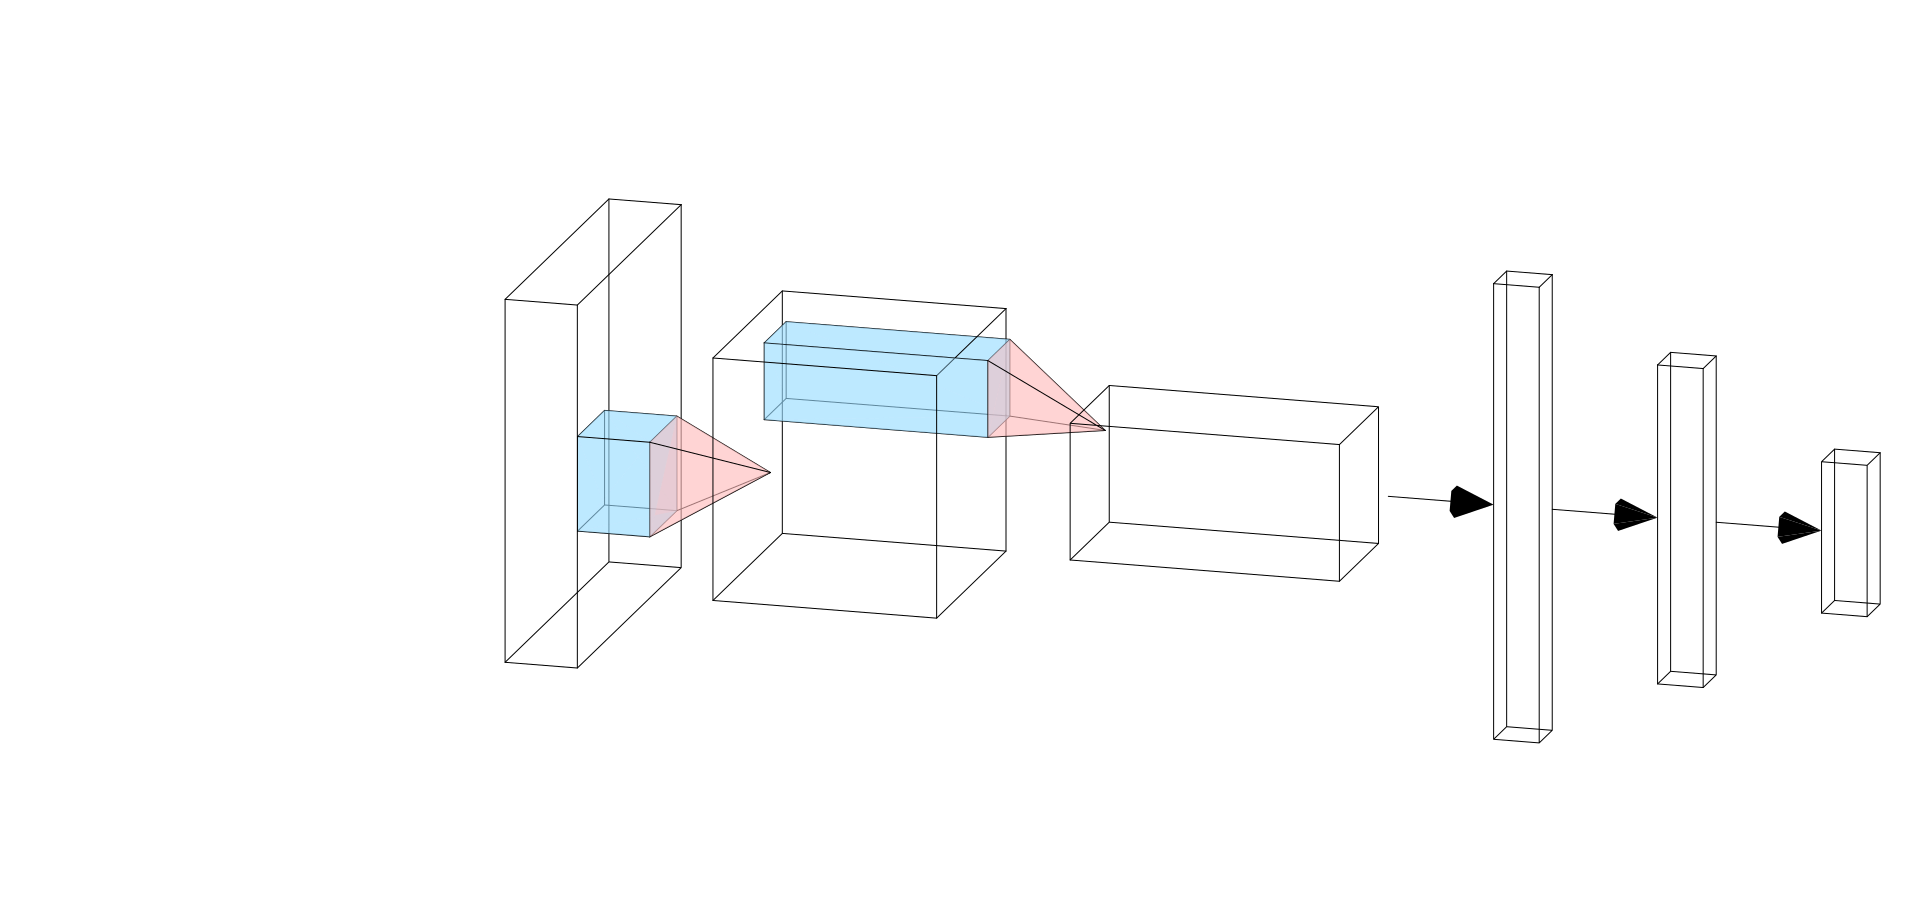
\includegraphics[width=16cm]{CNN}
\caption{Schéma du cerveau artificiel complet}
\end{figure}


\textbf{Cependant nous avons choisi} après de nombreuses heures de travail et de nombreux échecs lors de notre première version avec cette architecture, de l'\textbf{adapter et de modifier le concept de pooling} pour rendre l'intégration plus aisée. Elle sera \textbf{théoriquement moins efficace} qu'un pooling classique mais sera \textbf{réellement plus efficace} que notre implémentation du pooling classique grâce aux temps de calculs plus limités. Nous allons poser l'\textbf{hypothèse suivante}: \textbf{"Le concept de pooling est grossièrement approximable par une simple sélection arbitraire d'un pixel dans chaque carreau de notre image avant pooling}". Cette hypothèse réduit \textbf{légèrement la complexité de notre algorithme mais grandement celle du code}, il ne nous est donc plus utile de programmer les \textbf{fonctions de pooling qui s'avèrent très lourdes et compliquées à manipuler lors de la rétro-propagation}. Nous remplaçons donc le pooling par le Stride. Le \textbf{Stride }est qualifié avec un format $(sw, sh)$. Si l'on applique simplement notre hypothèse, nous devrions calculer des valeurs qui nous seraient inutiles, or on sait à l'avance quelles valeurs vont nous être utiles, nous pouvons donc encore réduire le nombre de calculs à effectuer en effectuant le strict minimum des opérations nécessaires. Le \textbf{Stride ici représente la répartition des valeurs que l'on va calculer dans l'image initiale}. Par exemple, si l'on choisi un Stride de format $(3,3)$ avec des kernel de format $(2,2)$ ou un stride de $(2,2)$ avec des kernel de $(3,3)$, nous obtenons les schémas suivants:\\
\begin{figure}[h]
\centering
\includegraphics[width=12cm]{Stride}
\caption{Schéma pour deux formats de kernel et de strides}
\end{figure}


Ici sur le \textbf{deuxième schéma}, on voit qu'une colonne et qu'une ligne de zéro ont été ajoutées sur les bordures de la matrice. En effet dans cet exemple, \textbf{pour appliquer le kernal, il faut adapter la méthode}: il y a deux solutions qui sont le \textbf{padding et l'overlapping}. Le \textbf{padding} consiste en \textbf{l'intégration de l'image initiale dans une plus grosse remplie de 0 de telle sorte que son format soit le plus petit plus grand applicable à la convolution}. \textbf{L'overlapping} quant à lui \textbf{modifie les emplacements d'application des kernel} en partie hors limites, pour leur donner les derniers emplacements viables. \\ \\
\indent Il est important de rappeler que dans tous les réseaux de neurones, les paramètres sont posés aléatoirement.\textbf{ Ici, les poids et les biais du DNN sont toujours des paramètres mais ils sont à présent accompagnés par les valeurs des composantes (poids) des nombreux kernel} qui composent notre CNN. Il faudra donc \textbf{compléter les équations de rétro-propagation} pour les adapter au CNN et ainsi permettre d'entraîner nos poids. 

\section{Évolution}
\subsection{Prolongement et adaptation de la rétro-propagation}
Pour entrainer notre algorithme, nous allons toujours utiliser \textbf{une base de données}. Les \textbf{idées générales} régissant l'algorithme d'apprentissage seront donc \textbf{en partie identiques}. Comme vu sur les schémas précédents, \bsc{Figure 13}, la structure de l'algorithme ce découpe en deux parties dont la seconde est celle d'un DNN. Lors de la \textbf{rétro-propagation}, on fait reculer l'erreur dans le réseau donc la \textbf{première partie de la rétro-propagation} est \textbf{déjà maitrisée}. Il n'y a plus qu'à \textbf{établir les relations de rétro-propagation dans le CNN}. 
\subsubsection{Les notations}
Définissons de nouvelles notations pour les influences des paramètres et valeurs du CNN sur l'erreur:
\begin{itemize}
\item $\ud A^l$ correspond à la matrice des influences de chaque valeur de $A^l$. Elle se détaille de la manière suivante: $\ud A^{l,n}_{w,h,d}$ si l'on considère qu'il s'agit de la matrice du $n$-ième élément du mini-batch.
\item $\ud Z^l$ correspond à la matrice des influences de chaque valeur de $Z^l$. Elle se détaille de la manière suivante: $\ud Z^{l,n}_{w,h,d}$ si l'on considère encore une fois la matrice du $n$-ième élément du mini-batch.
\item $\ud K^l$ correspond à la matrice des influences de chaque valeurs de $K^l$. Elle se détaille de la manière suivante: $\ud K^{l,i,n}_{w,h,d}$ si l'on considère encore une fois la matrice du $n$-ième élément du mini-batch. Ici, $i$ est l'indice du $i$-ème kernal de la couche.
\end{itemize}

\subsubsection{Les équations mathématiques}
Il est donc possible de trouver des équations mathématiques pour la rétro-propagation. Commençons par traiter \textbf{la jonction entre les deux formes d'algorithmes}. La dernière image en sortie du CNN est mise sous le format d'un vecteur avant d'être mise en entrée du DNN. Lorsque l'on aura grâce à la rétro-propagation obtenu \textbf{les influences $\ud a^0$, nous devrons les reformater de sorte à obtenir $\ud A^L$.} Ensuite, grâce à des \textbf{dérivées partielles, on rétro-propage l'erreur sur les paramètres et valeurs du CNN}. Les équations obtenues par dérivation (les démonstrations sont disponibles dans l'annexe) sont les suivantes:

\begin{align}
\ud Z^l &= \sigma '(Z^l) \cdot \ud A^{l+1} \\
\ud A^{l,n}_{w,h,d} &=  \sum_{k=0}^{kc^l-1}\sum_{x=\lfloor\frac{w-kw^l}{sw^l} \rfloor+1}^{\lfloor \frac{w}{sw^l} \rfloor}\sum_{y=\lfloor\frac{h-kh^l}{sl} \rfloor+1}^{\lfloor \frac{h}{sh^l} \rfloor}(\ud Z^{l,n}_{x,y,k}\cdot W^{l,k}_{w-x\cdot sw^l, h - y\cdot sh^l, d}) \\
\ud K^{l,c,n}_{w,h,d} &= \sum_{x=0}^{ \lceil \frac{W^l}{sw^l} \rceil} \sum_{y=0}^{\lceil \frac{H^l}{sh^l}\rceil }\ud Z^{l,n}_{x,y,c}\cdot A^{l,n}_{x\cdot sw^l+w, y\cdot sh^l+h, d}
\end{align}

\textbf{Ces quelles formules nous permettent ainsi de rétro-propager l'erreur dans tout l'algorithme et ainsi modifier les paramètres qui sont les poids, les biais et le contenu des kernel.} Mais, il faut \textbf{d'abord obtenir les gradients} de chaque paramètre en faisant la moyenne des influences selon les mini-batchs. La formule de moyenne est la suivantes, avec $n =$ nombre de batchs :
\begin{equation}
gp^l = \frac{1}{n}\sum_{k=0}^{n-1}\ud p^{l,n}
\end{equation}
La formules de modification des paramètres est la suivante:
\begin{equation}
p^l - \gamma \cdot gp^l \mapsto p^l
\end{equation}
Il reste à établir le processus d'apprentissage.

\subsubsection{L'algorithme d'apprentissage}

La rétro-propagation va se dérouler en plusieurs étape:
\begin{itemize}
\item Calcul de l'erreur en sortie du réseau de neurones.
\item Rétro-propagation de l'erreur sur l'ensemble des valeurs et paramètres du DNN.
\item Conversion de format de l'erreur du DNN au format de l'erreur de la dernière couche du CNN.
\item Pour chaque couche de CNN, on rétro-propage l'erreur en appliquant dans l'ordre la formule (18) pour obtenir $\ud Z^l$. Ces influences, grâce aux formules (19) et (20), nous permettent d'obtenir $\ud A^l$ et $\ud K^l$.
\item Calcul des gradients en effectuant la moyenne des influences selon les mini-batchs.
\item Modification des paramètres en fonction de ces gradients. 
\end{itemize}

\subsection{Algorithme final et Batch-Normalization}
Maintenant que la structure de l'algorithme et que l'apprentissage ont été établis, il nous faut essayer d'\textbf{optimiser nos performances}. Avec l'algorithme nu précédemment présenté, nous arrivions à atteindre les \textbf{100$\%$ de réussite sur les Trains de MNIST mais seulement 70$\%$ sur le trains} et cela prenait du temps, ce qui n'est \textbf{pas qualifiable de bon résultat}. Sur la base de données \textbf{CIFAR10}, une variante plus légère et facile de CIFAR15, les performances était de \textbf{70$\%$ sur les Trains} mais l'algorithme est très lent et un problème que l'on pensait en partie avoir réglé est réapparue, le \textbf{sur-apprentissage}. Nous obtenions des courbes similaires à la suivante: \\
\begin{figure}[h]
\centering
\includegraphics[height=5cm]{overfittingl}
\caption{Courbe d'illustration du sur-apprentissage}
\end{figure}
\newpage
Ici, l'on voit bien que les \textbf{performances} de l'algorithme sur les \textbf{Trains }ne cessent de \textbf{s'améliorer} mais à partir d'un certains nombres d'époques, les \textbf{performances sur les Tests} arrêtent de s'améliorer non pas pour tendre vers une asymptote horizontale \textbf{mais pour diverger}. Cela \textbf{engendre un algorithme} qui est \textbf{inutile} car il n'arrive pas à extraire une sémantique des informations qui lui sont fournies: \textbf{sa complexité est utilisée pour apprendre par cœur les données d'entrainement plutôt que de chercher une méthode d'analyse qui pourrait s'adapter à un plus grand nombres d'images}, ce qui est handicapant car il doit être en capacité de reconnaître des objets dans des positions qu'il risque de ne jamais avoir vu, dans des contextes qu'il n'a jamais vu. La dernière partie du projet se consacre donc à \textbf{régler au maximum le problème du sur-apprentissage}. Pour cela, nous allons utiliser une technologie appelée batch-normalisation.
\subsubsection*{La batch-normalization}
Ici, il faut réussir à \textbf{limiter le sur-apprentissage}. Sur des bases de données comme \textbf{MNIST}, où l'on reconnait des \textbf{chiffres écrits à la main}, il y a une \textbf{faible diversité d'images} pour chaque label. Alors que sur une base de données telle que \textbf{CIFAR}, où \textbf{deux images correspondant au même label peuvent être très éloignées}. 
 \begin{figure}[h]
    \begin{minipage}[c]{.46\linewidth}
        \centering
        \includegraphics[height=4.5cm]{mnist_exemple}
        \caption{Images issuent de MNIST}
    \end{minipage}
    \hfill%
    \begin{minipage}[c]{.46\linewidth}
        \centering
        \includegraphics[height=4.5cm]{CIFAR-10_examples}
        \caption{Images issuent de CIFAR 10}
    \end{minipage}
\end{figure}

\textbf{ Il nous faut donc réussir à "uniformiser" nos données}. C'est ce que propose la \textbf{Batch-normalisation} \cite{bn}. Elle ce base sur l'hypothèse que l'algorithme aurait plus de facilité à reconnaître un peu plus d'images si celle-ci avait une répartition statistique équivalente. \textbf{Pour résumer, la batch-normalisation va permettre à l'algorithme de se concentrer sur le fond et non la forme des données, cela rend donc l'apprentissage bien plus rapide et réduit le sur-apprentissage.} Cette technique se concentre grandement sur \textbf{l'utilisation des moyennes et des variances} de nos images. D'un point de vue technique, son implémentation est cependant plus complexe. Si l'on reprend le schéma global d'un CNN:
 \begin{figure}[h]
\centering
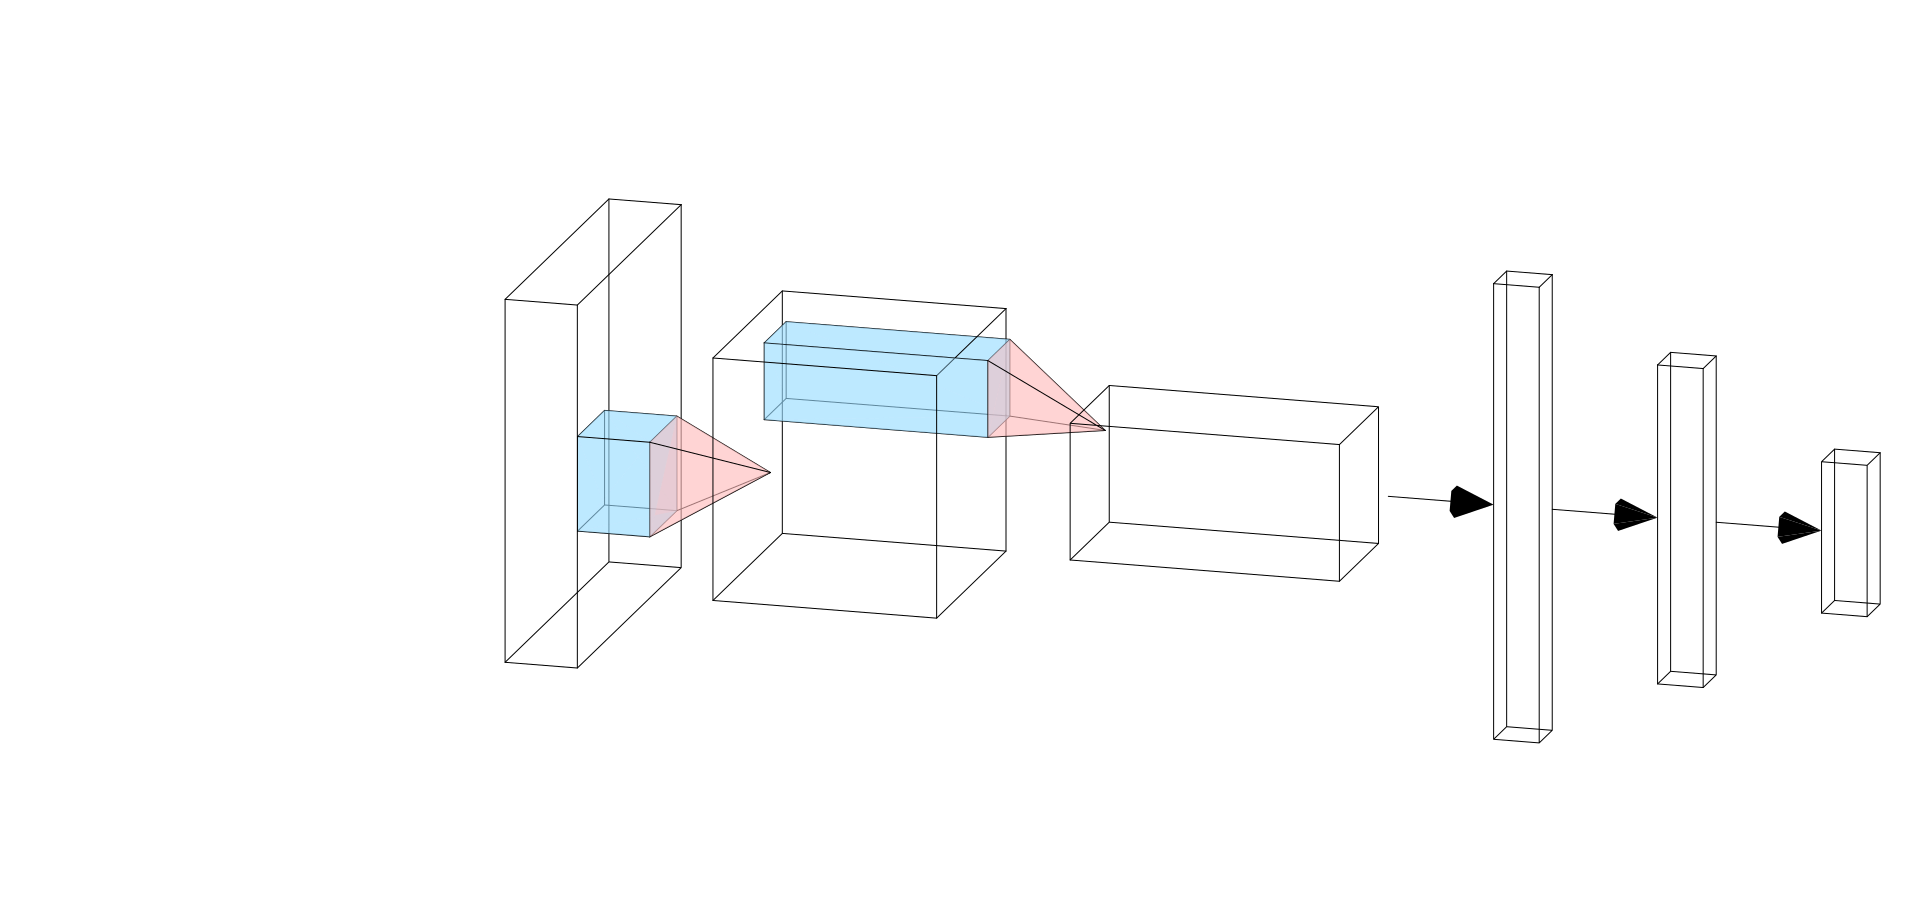
\includegraphics[width=16cm]{CNN}
\caption{Schéma du cerveau artificiel complet}
\end{figure}

Il nous faut \textbf{rajouter une étape} à l'entrée de chacune des couches. L'étape de normalisation. Cette étape va permettre \textbf{d'uniformiser l'entrée en ajustant sa moyenne et sa variance}. Elle va tout d'abord \textbf{centrer et réduire} statistiquement les entrées pour ensuite \textbf{choisir un nouvel écart type et une nouvelle moyenne}. Ces nouvelles répartitions statistiques que l'on va attribuer à chaque couche sont représentées par deux valeurs $ ba^l $ et $bg^l$, qui sont respectivement les moyennes et les écart-type de chaque couche. Les équations permettant des les appliquer sont les suivantes:
\begin{align}
<n^l>&=\frac{1}{Card(n^l)}\cdot\sum_{k\in n^l}k \\
z^l_k &=\frac{n^l_k-<n^l>}{\sqrt{\sum_{k\in n^l}(k-<n^l>)^2+\epsilon}}\cdot bg^l + ba^l
\end{align}
Cette étape se situe plus précisément entre le calcul principal de chaque couche et la fonction d'activation qui le suit. On appelle donc $n^l$ l'image de $a^l$ par notre calcul principal, et on a $z^l$ l'image de $n^l$ par la normalisation. Il faut donc établir les équations de rétro-propagation sur cette étape; ici, les paramètres sont $ ba^l $ et $bg^l$. \textbf{Il faut donc 3 nouvelles équations de rétro-propagation :}

\begin{align}
\ud n^l_k &= \frac{bg^l}{sqrt{\sum_{k\in n^l}(k-<n^l>)^2+\epsilon}}\cdot \ud z^l_k \\
\ud bg^l &= \sum_k \frac{n^l_k-<n^l>}{\sqrt{\sum_{k\in n^l}(k-<n^l>)^2+\epsilon}}\cdot \ud z^l_k \\
\ud ba^l &= \sum_k \ud z^l_k
\end{align}

Elles sont obtenues de la même manière, en appliquant les \textbf{dérivées partielles} sur chaque expression selon le paramètre voulu. (Démonstration dans l'annexe)

Maintenant que l'architecture est complète, nous pouvons procéder aux tests et chercher à comprendre les performances de l'algorithme.

\section{Résultats}

Nous avons \textbf{testé de nombreuses configurations} pour le CNN et le DNN en \textbf{faisant varier}:
\begin{itemize}
\item Pour le CNN:
	\begin{itemize}
	\item Le nombre de couches 
	\item Le nombre de kernel par couche
	\item Le format des kernel sur chaque couche
	\item Le format des strides sur chaque couche

	\end{itemize}
\item Pour le DNN:
	\begin{itemize}
	\item Le nombre de couches
	\item Le nombre de neurones par couche
	\end{itemize}
\item Les hyper-paramètres:
	\begin{itemize}
	\item les fonctions d'activation
	\item Ceux des optimiseurs
	\item Ceux des modifications des paramètres
	\item L'aléatoire initial
	\end{itemize}
\end{itemize}

Cela nous a amené après de très \textbf{nombreux tests} à une configuration que nous avons considérée \textbf{suffisamment performante} pour répondre à notre problème.

Il s'agit de la configuration suivante:
\begin{itemize}
\item Pour le CNN:
	\begin{itemize}
	\item 2 couches
	\item Respectivement 6 et 12
	\item Respectivement (4,4) et (3,3)
	\item Respectivement (3,3) et (2,2)

	\end{itemize}
\item Pour le DNN:
	\begin{itemize}
	\item 3 couches
	\item Respectivement 275, 48 et 15 de l'entrée à la sortie 
	\end{itemize}
\item Pour les hyper-paramètres:
	\begin{itemize}
	\item RELU sauf pour la sortie en Softmax
	\item Drop out 0.2 sur DNN, Momentum pour l'optimiseur, 0.9 pour le paramètre du momentum
	\item Utilisation de taux qui varie sur tout la durée de l'entrainement de manière sinusoïdale (de sortes que l'ensemble de l'entrainement corresponde à $ [0 ,\pi ]$ ); la taille des mini-batchs est de 128.
	\end{itemize}
\end{itemize}

Avec cette configuration, \textbf{les résultats sur CIFAR15 ont évolué jusqu'à atteindre les 42\% de réussite(Tests) en seulement 4 minutes d'entrainement}. Maintenant, si l'on prend en compte (en plus de la sortie de l'algorithme) le second résultat le plus probable, on se rend compte que l'algorithme à des performances atteignant les 70\% de réussite. \textbf{Cela est très convenable. En sachant que de nombreuses technologies plus performantes n'ont pas été intégrées à l'algorithme car nous ne les comprenions pas, nous pourrions espérer dans un futur proche atteindre les 60 \% de réussite en nous penchant plus sérieusement sur ces méthodes.} La batch-normalisation nous a donc permis d'augmenter de 15\% les performances de l'algorithme sur CIFAR15. Elle nous a en partie permis de \textbf{contourner le problème de diversification}, causé entre autre par la faible quantité de données disponibles pour l'entrainement et de la grande diversité de celle-ci, qui ne permet pas de convenir convenablement l'entièreté de chaque catégorie. 
 \begin{figure}[h]
\centering
\includegraphics[width=16cm]{answer_to_life_m}
\caption{Performance durant l'entrainement sur CIFAR15}
\end{figure}
\newpage
Maintenant que nous avons un \textbf{algorithme "performant"}, nous avons voulu nous attaquer à un nouveaux problème. Sur la base de donnée \textbf{CIFAR100}, deux types de labels sont disponibles. Le premier, \textbf{le plus précis}, classe précisément chaque image dans une des \textbf{100 sous catégories} de la base de données. \textbf{Le second, plus généraliste }regroupe les \textbf{100 sous catégories sous 20 catégories plus larges}.

\begin{figure}[h]
\centering
\includegraphics[width=14.5cm]{categorie_CIFAR100}
\caption{Ensemble des catégories et sous catégories de CIFAR100}
\end{figure}

Essayer de faire de \textbf{la reconnaissance} sur ces 20 catégories s'est avéré \textbf{très intéressant}, puisque malgré \textbf{la grande quantité de données, la diversité de celles-ci est énorme, et il sera donc difficiles d'obtenir de bons résultats}.

\textbf{Les résultats} obtenus après avoir trouvé les bons réglages \textbf{paraissent médiocres}, 12\% de réussite. \textbf{Cependant nous avons été agréablement surpris en constatant que, oui les résultats n'étaient pas parfaits, mais l'algorithme avait réussi à obtenir une compréhension sémantique de la base données.} Par exemple, quand on lui montrait une \textbf{image d'homme}, \textbf{il renvoyait à l'ordre près: people, medium-sized mammals et large omnivores and herbivores}, alors qu'il était \textbf{seulement entrainé à reconnaître people}. Cela témoigne qu'il arrive à \textbf{obtenir un comportement pour lequel il n'a pas été entrainé}. Cela a été un \textbf{moment clef} de notre projet: pour la première fois, un \textbf{comportement inattendu a émergé}, qui de plus était correct. Cela montre la puissance de cette technologie. 

\textbf{Nous avons terminé l'exploration de cette branche de l'intelligence artificielle} sur cette réussite. Dans le futur,\textbf{ nous allons nous concentrer sur une nouvelle branche qui permet de faire de la prise de décision}.

\part{Conclusion Générale}

\textbf{À notre problématique, nous avons trouvé une solution technique}. Cet algorithme de reconnaissance d'images fait appel à de \textbf{nombreuses thématiques technologiques de notre temps}: l'accès à une grande quantité d'images avec le \textbf{bigdata}, la capacité de calculs avec les \textbf{super ordinateurs}, et pour finir l'\textbf{intelligence artificielle}. Durant ce projet, nous avons appris et en partie compris le fonctionnement d'une intelligence artificielle fonctionnant avec un apprentissage supervisé. Nous avons réussi à obtenir des résultats sur différentes bases de données très diverses, de difficultés variées. Nous avons fait évoluer nos algorithmes pour qu'ils correspondent aux besoins que nous avions. Il est vrai, nous aurions pu avec plus de temps nous intéresser à d'autres types d'algorithmes de deep learning permettant de faciliter la reconnaissance d'images, nous aurions pu nous intéresser à d'autres optimiseurs, et un grand nombre de facettes de la reconnaissance d'images reste à explorer. \textbf{Ce projet nous a permis de nous donner des bases solides nous permettant de nous atteler à de nouveaux projets, et nous allons dès à présent concentrer notre travail sur les algorithmes de prises de décisions, avec comme objectif de faire apprendre à nager à un modèle 3D}. 

\newpage 

\bibliographystyle{plain}
\bibliography{data_base}

\newpage
\part{Preuves}
\section{Démonstration des équations de la rétro-propagation DNN}

Démontrons par récurrence la rétro-propagation, c'est-à-dire qu'il est possible de définir l'influence de chacune des valeurs définies par chaque notation sur la fonction $E$: \\
Rappelons l'expression de la fonction erreur:
\[E=(Y^*-y)^2\Leftrightarrow E = <(Y^*-y)|(Y^*-y)> \Leftrightarrow E = \sum_k(Y^*_k-a^L_k)^2 \]
\textbf{Initialisation:} \\ 
\indent On peut en déduire l'influence de la dernière couche sur la sortie en utilisant une dérivée partielle.
\[\ud a^L_k=\frac{\partial E}{\partial a^L_k}=a^L_k-2Y^*_k\]
À partir de maintenant, nous allons trouver des formules mathématiques permettant de répandre de manière récursive l'influence de l'erreur.\\ \\
\textbf{Hérédité:}\\
\indent Supposons qu'il existe l tel que l'on connaisse $da^l$, et essayons de calculer $da^{l-1}$.
Nous pouvons tout d'abord calculer l'influence de $z$ sur l'erreur:
\[\ud z^l_k=\frac{\partial E}{\partial z^l_k}=\frac{\partial E}{\partial a^l_k}\cdot \frac{\partial a^l_k}{\partial z^l_k}=\sigma'(z^l_k)\ud a^l_k\]
Il nous faut maintenant avoir l'influence de $a^{l-1}$ sur $E$:
\[\ud a^{l-1}_k=\frac{\partial E}{\partial a^{l-1}_k}=\frac{\partial E}{\partial z^l}\cdot\frac{\partial z^l}{\partial a^{l-1}_k}=\sum_i  w^l_{i,k}\ud z^l_i\]
Il nous reste donc à calculer l'influence des poids et biais sur l'erreur :\\
\begin{itemize}
\item Pour les poids :
\[\ud w^l_{i,k}=\frac{\partial E}{\partial w^l_{n,k}}=\frac{\partial E}{\partial z^l_k}\cdot \frac{\partial z^l_k}{\partial w^l_{n,k}}=a^{l-1}_i\ud z^l_k\]
\item Pour les biais :
\[\ud b^l_k=\frac{\partial E}{\partial b^l_k}=\frac{\partial E}{\partial z^l_k}\cdot \frac{\partial z^l_k}{\partial b^l_k}=\ud z^l_k\]
\end{itemize} 
\textbf{Conclusion:}\\
\indent D'après le principe de récurrence, on peut en déduire que les influences sont en effet rétro-propageables sur l'ensemble du réseau de neurones.\\

\section{Démonstration des équations de la rétro-propagation CNN}
Démontrons par récurrence la rétro-propagation dans le CNN. La propriété $P_l$ est la suivante: Si l'on connait l'influence de la couche l sur l'erreur alors il est possible de connaître l'influence de la couche $l-1$.\\ \\
\textbf{Initialisation:}\\
\indent On connait l'influence de la sortie de la dernière couche du CNN grâce à la rétro-propagation sur le DNN.
On connait donc $P_L$.\\ \\
\textbf{Hérédité:}\\
\indent Supposons qu'il existe $l\in \ldbrack 2, L \rdbrack$ tel que $P_l$ soit vraie. Montrons que la propriété est vraie au rang $l-1$\\
\begin{itemize}
\item La fonction d'activation:\\
\begin{align}
		\ud Z^{l-1,n}_{w,h,d}&=\frac{\partial E}{\partial Z^{l-1,n}_{w,h,d}} \\
		\ud Z^{l-1,n}_{w,h,d}&=\frac{\partial E}{\partial A^{l,n}_{w,h,d}}\cdot \frac{\partial A^{l,n}_{w,h,d}}{\partial Z^{l-1,n}_{w,h,d}} \\
		\ud Z^{l-1,n}_{w,h,d}&=\sigma '(Z^{l-1,n}_{w,h,d}) \cdot \ud A^{l,n}_{w,h,d}
\end{align}
On peut ici vectoriser l'expression pour la rendre plus lisible:
\begin{equation}
\ud Z^{l-1} = \sigma '(Z^{l-1}) \cdot \ud A^{l}
\end{equation}


\item Le produit de convolution:\\
\begin{align}		
		\ud A^{l-1,n}_{w,h,d} &= \frac{\partial E}{\partial A^{l-1,n}_{w,h,d}} \\
		\ud A^{l-1,n}_{w,h,d}&=\frac{\partial E}{\partial Z^{l-1,n}_{w,h,d}}\cdot \frac{\partial Z^{l-1,n}_{w,h,d}}{\partial A^{l-1,n}_{w,h,d}} \\
		\ud A^{l-1,n}_{w,h,d}&=\frac{\partial Z^{l-1,n}_{w,h,d}}{\partial A^{l-1,n}_{w,h,d}} \cdot \ud Z^{l-1,n}_{w,h,d} 
\end{align}
Ce formalise ici ne marche pas car les valeurs de $A^{l-1,n}$ s'applique sur de nombreuses valeurs de $\ud Z^{l-1,n}_{w,h,d}$, mais pour une seule application de la valeur de $A^{l-1,n}$, cela fonctionne. 
Il faut maintenant réussir à obtenir l'expression de $\frac{\partial Z^{l-1,n}_{w,h,d}}{\partial A^{l-1,n}_{w,h,d}}$.
Tout d'abord, chaque valeur $A^{l-1,n}_{w,h,d}$ est impliquée dans un certain nombre de fois le même calcul, nous allons donc trouver son expression pour un de ces calculs, puis il faudra sommer pour les prendre tous en compte. Ce simple calcul est un produit entre un poids qui s'applique sur la valeur (dont on cherche l'influence) et l'influence de la valeur qui a été calculée avec ce poids. Il nous faut ensuite sommer en faisant varier le poids, cela s'effectue en sommant sur les différents kernel de la couche et sommer sur les différentes influences $\ud Z^{l-1,n}$ qui utilise $A^{l-1,n}_{w,h,d}$ pour être calculées.
Cela nous donne la formule suivante:
\begin{align}
	\ud A^{l-1,n}_{w,h,d}&=\frac{\partial Z^{l-1,n}_{w,h,d}}{\partial A^{l-1,n}_{w,h,d}} \cdot \ud Z^{l-1,n}_{w,h,d} \\
	\ud A^{l-1,n}_{w,h,d} &=  \sum_{k=0}^{kc^{l-1}-1}\sum_{x=\lfloor\frac{w-kw^{l-1}}{sw^{l-1}} \rfloor+1}^{\lfloor \frac{w}{sw^{l-1}} \rfloor}\sum_{y=\lfloor\frac{h-kh^{l-1}}{sl^{l-1}} \rfloor+1}^{\lfloor \frac{h}{sh^{l-1}} \rfloor}(\ud Z^{l-1,n}_{x,y,k}\cdot W^{l-1,k}_{w-x\cdot sw^{l-1}, h - y\cdot sh^{l-1}, d})
\end{align}

\item Les poids des kernel:\\
\begin{align}
\ud K^{l-1,c,n}_{w,h,d} &= \frac{\partial E}{\partial K^{l-1,c,n}_{w,h,d}} \\
		\ud K^{l-1,c,n}_{w,h,d}&=\frac{\partial E}{\partial Z^{l-1,n}_{w,h,d}}\cdot \frac{\partial Z^{l-1,n}_{w,h,d}}{\partial K^{l-1,c,n}_{w,h,d}} \\
		\ud K^{l-1,c,n}_{w,h,d}&=\frac{\partial Z^{l-1,n}_{w,h,d}}{\partial K^{l-1,c,n}_{w,h,d}} \cdot \ud Z^{l-1,n}_{w,h,d}
\end{align}
Ce formalise ici ne marche pas car les poids s'applique sur de nombreuses valeurs de $\ud Z^{l-1,n}_{w,h,d}$, mais pour une seule application de celui-ci, cela fonctionne. 
Pour obtenir l'expression de $\frac{\partial Z^{l-1,n}_{w,h,d}}{\partial K^{l-1,c,n}_{w,h,d}}$ il faut procéder de la même manière que précédemment. Pour un calcul, l'expression sera le produit d'une des influences de $\ud Z^{l-1,n}$ par la valeur de $A^{l-1,n}$ qui correspondant. Il faut ensuite sommer tout ça pour couvrir toute les applications du poids. Pour cela on somme sur les emplacement du kernal durant le produit de convolution. Cela nous donne la formule suivante:


\begin{align}
	\ud K^{l-1,c,n}_{w,h,d}&=\frac{\partial Z^{l-1,n}_{w,h,d}}{\partial K^{l-1,c,n}_{w,h,d}} \cdot \ud Z^{l-1,n}_{w,h,d} \\
	\ud K^{l-1,c,n}_{w,h,d} &= \sum_{x=0}^{ \lceil \frac{W^{l-1}}{sw^{l-1}} \rceil} \sum_{y=0}^{\lceil \frac{H^{l-1}}{sh^{l-1}}\rceil }\ud Z^{l-1,n}_{x,y,c}\cdot A^{l-1,n}_{x\cdot sw^{l-1}+w, y\cdot sh^{l-1}+h, d}	
\end{align}
\end{itemize}
\textbf{Conclusion:} \\
\indent Par le principe de récurrence, on peut conclure que l'erreur est bien rétro-propageable sur l'ensemble du CNN. Cela nous permet donc d'obtenir une rétro-propagation complète sur l'ensemble du réseau de neurones. 
\newpage
\section{Démonstration des équations de rétro-propagation  Batch-normalisation} 

Démontrons la propriété suivantes, il est possible de rétro-propager l'erreur sur les zones de normalisation.\\

On connait les valeurs des influences $\ud z^l_k$. En dérivant selon $n^l$ l'expression suivante \\ $\frac{n^l_k-<n^l>}{\sqrt{\sum_{k\in n^l}(k-<n^l>)^2+\epsilon}}\cdot bg^l + ba^l$ on obtient l'expression $\frac{bg^l}{\sqrt{\sum_{k\in n^l}(k-<n^l>)^2+\epsilon}}$. En sachant que l'on a l'équivalence suivante:
\begin{equation}
\ud n^l_k = \frac{\partial E}{\partial n^l_k} \Leftrightarrow \ud n^l_k = \frac{\partial E}{\partial z^l_k}\cdot \frac{\partial z^l_k}{\partial n^l_k}=\frac{\partial z^l_k}{\partial n^l_k}\cdot \ud z^l_k
\end{equation}
On peut ensuite remplacer $\frac{\partial z^l_k}{\partial n^l_k}$ par l'expression obtenu précédemment:
\begin{equation}
\ud n^l_k = \frac{bg^l}{\sqrt{\sum_{k\in n^l}(k-<n^l>)^2+\epsilon}}\cdot \ud z^l_k
\end{equation}
En vectorisant les expressions, on arrive à l'expression suivante:
\begin{equation}
\ud n^l = \frac{bg^l}{\sqrt{\sum_{k\in n^l}(k-<n^l>)^2+\epsilon}}\cdot \ud z^l
\end{equation}
On a ensuite, de manière assez aisée, l'influence du paramètre de moyenne. Lorsque l'on dérive $\frac{n^l_k-<n^l>}{\sqrt{\sum_{k\in n^l}(k-<n^l>)^2+\epsilon}}\cdot bg^l + ba^l $ selon $ba^l $, le résultat vaut $1$. Si l'on effectue la même dérivation sur  $ \frac{n^l-<n^l>}{\sqrt{\sum_{k\in n^l}(k-<n^l>)^2+\epsilon}}\cdot bg^l + ba^l $, on obtient un vecteur du même format que $z^l$ remplit de $1$. Or on a le résultat suivant:
\begin{align}
\ud ba^l &= \frac{\partial E}{\partial ba^l}\\
\ud ba^l &= \frac{\partial E}{\partial z^l}\cdot\frac{\partial z^l}{\partial ba^l} \\
\ud ba^l &= \frac{\partial z^l}{\partial ba^l}\cdot \ud z^l 
\end{align}
On peut remplacer $\frac{\partial z^l}{\partial ba^l}$ par un vecteur remplit de $1$, ce qui nous donne donc le produit scalaire qui somme les composante de $z^l$:
\begin{align}
\ud ba^l &= \frac{\partial z^l}{\partial ba^l}\cdot \ud z^l \\
\ud ba^l &= \sum_k \ud z^l_k
\end{align}
il nous reste à calculer l'influence du paramètre gérant l'écart type. Lorsque l'on  \\ dérive $\frac{n^l-<n^l>}{\sqrt{\sum_{k\in n^l}(k-<n^l>)^2+\epsilon}}\cdot bg^l + ba^l$ selon $bg^l$, on obtient le vecteur dont les composantes sont $\forall k, \frac{n^l-<n^l>}{\sqrt{\sum_{k\in n^l}(k-<n^l>)^2+\epsilon}}\cdot bg^l + ba^l$. De même que pour les influences précédentes:
\begin{align}
\ud bg^l &= \frac{\partial E}{\partial bg^l} \\
\ud bg^l &= \frac{\partial E}{\partial z^l}\cdot\frac{\partial z^l}{\partial bg^l}  \\
\ud bg^l &= \frac{\partial z^l}{\partial bg^l}\cdot \ud z^l 
\end{align}
Ici on a de même un produit scalaire, qui se développe et nous donne:
\begin{align}
\ud bg^l &= \frac{\partial z^l}{\partial bg^l}\cdot \ud z^l \\
\ud bg^l &= \sum_k \frac{n^l_k-<n^l>}{\sqrt{\sum_{k\in n^l}(k-<n^l>)^2+\epsilon}}\cdot \ud z^l_k 
\end{align}

\newpage


\part{Algorithmes:}
\section{Algorithme interface et sauvegarde:}
\lstset{language=Python}
\begin{lstlisting}[mathescape]
""" Main program -- manage UI and convolutional neural network """

import pickle
import numpy as np
import matplotlib.pyplot as plt
import convolutional_neural_network as cnn

" Set hyper-parameters "

save_name = ''
save_type = 'test'
data_set_name = 'cifar_100_coarse'
count = 20
inputs_dimensions = (32, 32, 3)

cnn_topology = {'Lc': 2,
                'kc1': 6, 'kc2': 12,
                'kd1': (4, 4), 'kd2': (3, 3),
                'sc1': (3, 3), 'sc2': (2, 2),
                'afc1': 'relu', 'afc2': 'relu',
                }
dnn_topology = {'Ld': 2,
                'nc1': 48, 'nc2': count,
                'afd1': 'relu', 'afd2': 'softmax',
                'dor0': 0.2, 'dor1': 0.2
                }

epoch_count = 16
mini_batch_size = 256
optimizer = 'momentum'
alpha = '0.6 + 0.4 * math.sin(math.pi * t)'
beta = '0.95 - 0.05 * math.sin(math.pi * t)'
gamma = '0.9'
rho = '0.9'
lambda2C = 0.01
lambda2D = 0.1
training_count = 50000
testing_count = 5000

data = pickle.load(open(data_set_name, 'rb'))
training = (data['train_x'][:, :, :, :training_count], data['train_y'][:, :training_count])
testing = (data['test_x'][:, :, :, :training_count], data['test_y'][:, :training_count])
labels = data['labels']

" Get parameters "

if save_name == '':

    arg = (cnn_topology, dnn_topology, inputs_dimensions)
    parameters = cnn.initialize_parameters(*arg)

    print('node_count_dnn_0:', parameters['nc0'])

    arg = (parameters, epoch_count, mini_batch_size, optimizer, alpha, beta, gamma, rho, lambda2C, lambda2D, training, testing, save_type)
    parameters, name, best_cost = cnn.train(*arg)

    hyper_parameters = {'cnn_topology': cnn_topology, 'dnn_topology': dnn_topology,
                        'epoch_count': epoch_count, 'mini_batch_size': mini_batch_size,
                        'optimizer': optimizer, 'alpha': alpha, 'beta': beta,
                        'gamma': gamma, 'rho': rho, 'lambda2C': lambda2C, 'lambda2D': lambda2D,
                        'best_cost': best_cost, 'training_count': training_count,
                        'testing_count': testing_count, 'save_type': save_type}
    save = {'parameters': parameters, 'hyper_parameters': hyper_parameters}
    pickle.dump(save, open(data_set_name+'_'+name, 'wb'))

else:

    save = pickle.load(open(save_name, 'rb'))
    parameters = save['parameters']
    print(save['hyper_parameters'])

    test_x, test_y = testing
    permutation = list(np.random.permutation(np.arange(testing_count, dtype=np.int16)))
    shuffled_x = test_x[:, :, :, permutation]
    shuffled_y = test_y[:, permutation]

    for i in range(testing_count):
        img = shuffled_x[:, :, :, i].reshape(inputs_dimensions + (1, ))
        goal = list(shuffled_y[:, i]).index(1)
        prediction = cnn.predict(parameters, img)

        result = {labels[k]: round(float(prediction[k]) * 100, 2) for k in range(count)}

        print(sorted(result.items(), key=lambda z: z[1], reverse=True))
        print(labels[goal])

        plt.close()
        plt.imshow(np.squeeze(img))
        plt.show()
\end{lstlisting}
\newpage
\section{Algorithme d'exécution du réseau de neurones}
\lstset{language=Python}
\begin{lstlisting}[mathescape]
import time
import math
import numpy as np
from copy import deepcopy
import matplotlib.pyplot as plt

def forward(parameters, x, masks=None):
    """
    Apply a forward propagation in order to compute cache

    Take :
    parameters -- dictionary containing all the information about the whole network
    x -- features (w, h, d, n)
    masks -- dropout's mask

    Return :
    cache -- dictionary of results
    """

    n = x.shape[3]
    cache = {'xc0': x}

    g = parameters['gc0']
    b = parameters['bc0']
    xh, a, v, m = normalize(x, g, b)
    cache['xhc0'] = xh
    cache['ac0'] = a
    cache['vc0'] = v
    cache['mc0'] = m

    for l in range(1, parameters['Lc'] + 1):
        w = parameters['wc' + str(l)]
        rc = parameters['rc' + str(l)]
        x = convolve(a, w, rc)
        cache['xc' + str(l)] = x

        g = parameters['gc' + str(l)]
        b = parameters['bc' + str(l)]
        xh, z, v, m = normalize(x, g, b)
        cache['xhc' + str(l)] = xh
        cache['zc' + str(l)] = z
        cache['vc' + str(l)] = v
        cache['mc' + str(l)] = m

        af = parameters['afc' + str(l)]
        if af == 'relu':
            a = relu(z)
        elif af == 'tanh':
            a = tanh(z)
        elif af == 'sigmoid':
            a = sigmoid(z)
        cache['ac' + str(l)] = a

    a = a.reshape(-1, n)
    cache['ad0'] = a

    if masks is not None:
        a *= masks[0]

    for l in range(1, parameters['Ld'] + 1):
        w = parameters['wd' + str(l)]
        x = np.dot(w, a)
        cache['xd' + str(l)] = x

        g = parameters['gd' + str(l)]
        b = parameters['bd' + str(l)]
        xh, z, v, m = normalize(x, g, b)
        cache['xhd' + str(l)] = xh
        cache['zd' + str(l)] = z
        cache['vd' + str(l)] = v
        cache['md' + str(l)] = m

        af = parameters['afd' + str(l)]
        if af == 'relu':
            a = relu(z)
        elif af == 'softmax':
            a = softmax(z)
        elif af == 'tanh':
            a = tanh(z)
        elif af == 'sigmoid':
            a = sigmoid(z)

        if masks is not None and masks[l] is not None:
            a *= masks[l]

        cache['ad' + str(l)] = a

    return cache
    
def convolve(A, W, rc):
    """
    Apply weights and biases on A

    Take :
    A -- numpy matrix, non linear values of the previous layer (w_A, h_A, d, n)
    W -- numpy matrix, weights to apply (count, w_W, h_W, d, 1)
    rc -- tuple, range of values of w and h

    Return :
    Z -- numpy matrix, linear values of the current layer (w_Z, h_Z, count, n)
    """

    lx, ly = rc
    tx, ty = len(lx), len(ly)
    count, w_W, h_W, _, _ = W.shape
    Z = np.zeros((tx, ty, count, A.shape[3]))

    for k in range(count):
        for x in range(tx):
            for y in range(ty):
                w, h = lx[x], ly[y]
                Z[x, y, k] += np.sum(A[w:w+w_W, h:h+h_W] * W[k], axis=(0, 1, 2))

    return Z

\end{lstlisting}
\newpage
\section{Algorithme de rétro-propagation}
\lstset{language=Python}
\begin{lstlisting}[mathescape]

import time
import math
import numpy as np
from copy import deepcopy
import matplotlib.pyplot as plt

def backward(parameters, y, cache, lambda2C=0, lambda2D=0):
    """
    Apply a backward propagation in order to compute gradients

    Take :
    parameters -- dictionary containing all the information about the whole network
    y -- labels (v, n)
    cache -- dictionary of results
    lambda2C -- L2 regularization rate for cnn
    lambda2D -- L2 regularization rate for dnn

    Return :
    gradients -- partial derivative of each parameters with respect to cost
    """

    gradients = {}
    n = y.shape[1]

    y_hat = cache['ad' + str(parameters['Ld'])]
    da = np.divide(1 - y, 1 - y_hat) - np.divide(y, y_hat)
    dz = None

    for l in reversed(range(1, parameters['Ld'] + 1)):
        z = cache['zd' + str(l)]
        af = parameters['afd' + str(l)]

        if af == 'relu':
            dz = da * relu_prime(z)
        elif af == 'softmax':
            dz = y_hat - y
        elif af == 'tanh':
            dz = da * tanh_prime(z)
        elif af == 'sigmoid':
            dz = da * sigmoid_prime(z)

        g = parameters['gd' + str(l)]
        x_p = cache['xd' + str(l)]
        xh_p = cache['xhd' + str(l)]
        v = cache['vd' + str(l)]
        m = cache['md' + str(l)]
        dz, dg, db = normalize_prime(dz, g, x_p, xh_p, v, m)
        gradients['dgd' + str(l)] = dg
        gradients['dbd' + str(l)] = db

        a_p = cache['ad' + str(l - 1)]
        w = parameters['wd' + str(l)]
        gradients['dwd' + str(l)] = (1 / n) * (np.dot(dz, a_p.T) + lambda2D * np.power(w, 2))

        da = np.dot(w.T, dz)

    da = da.reshape(cache['ac' + str(parameters['Lc'])].shape)

    for l in reversed(range(1, parameters['Lc'] + 1)):
        z = cache['zc' + str(l)]
        af = parameters['afc' + str(l)]

        if af == 'relu':
            dz = da * relu_prime(z)
        elif af == 'tanh':
            dz = da * tanh_prime(z)
        elif af == 'sigmoid':
            dz = da * sigmoid_prime(z)

        g = parameters['gc' + str(l)]
        x_p = cache['xc' + str(l)]
        xh_p = cache['xhc' + str(l)]
        v = cache['vc' + str(l)]
        m = cache['mc' + str(l)]
        dx, dg, db = normalize_prime(dz, g, x_p, xh_p, v, m)
        gradients['dgc' + str(l)] = dg
        gradients['dbc' + str(l)] = db

        a_p = cache['ac' + str(l - 1)]
        w = parameters['wc' + str(l)]
        rc = parameters['rc' + str(l)]
        da, dw = deconvolve(dx, w, a_p, rc)

        gradients['dwc' + str(l)] = (1 / n) * (dw + lambda2C * np.power(w, 2))

    g = parameters['gc0']
    x_p = cache['xc0']
    xh_p = cache['xhc0']
    v = cache['vc0']
    m = cache['mc0']
    dx, dg, db = normalize_prime(da, g, x_p, xh_p, v, m)
    gradients['dgc0'] = dg
    gradients['dbc0'] = db

    gradients['dxc0'] = dx

    return gradients
    
def deconvolve(dZ, W, A_p, rc):
    """
    Compute gradients

    Take :
    dZ -- numpy matrix, gradients of the next layer (w_dZ, h_dZ, count, n)
    W -- numpy matrix, weights (count, w_W, h_W, d, 1)
    A_p -- previous A (w_dA, h_dA, d, n)
    rc -- range of values of w and h

    Return :
    dA -- numpy matrix, gradients of the current layer (w_dA, h_dA, d, n)
    dW -- numpy matrix, weights gradients (count, w_W, h_W, d)
    db -- numpy matrix, biases gradients (1, 1, count, 1)
    """

    lx, ly = rc
    w_dZ, h_dZ, count, n = dZ.shape
    _, w_W, h_W, _, _ = W.shape

    dA = np.zeros_like(A_p)
    dW = np.zeros_like(W)

    for k in range(count):
        for x in range(w_dZ):
            for y in range(h_dZ):
                w, h, dZ_n = lx[x], ly[y], dZ[x, y, k].reshape(1, 1, 1, n)
                dA[w:w+w_W, h:h+h_W] += W[k] * dZ_n
                dW[k] += np.sum(A_p[w:w+w_W, h:h+h_W] * dZ_n, axis=3, keepdims=True)

    return dA, dW
\end{lstlisting}
\end{document}